% Include header.tex with configuration

%document class
\documentclass[
	accentcolor=tud9c,
	bibliography=totoc,
	twoside,
	numbersubsubsec,
	fontsize=12pt,
	type=msc,
	colorback,
	english
]{tudthesis}

% to-do notes
\usepackage[english]{todonotes}

% no identation for new paragraphs
\setlength{\parindent}{0pt}

% input encoding
\usepackage[utf8]{inputenc}
 	
% font encoding
\usepackage[T1]{fontenc}

% english document
\usepackage[english]{babel}

% set line spacing to 1.5
\usepackage{setspace}
\onehalfspacing

%hyperredf package
\usepackage{hyperref}

% multiple rows inside a table
%\usepackage{mutlirow}

% english quotes and package important for biblatex
\usepackage[english=british]{csquotes}

% consistent text for graphics
\usepackage{psfrag}

%package for matrix
\usepackage{amsmath}

%packages taken from sebastian thesis.tex
\usepackage{listings}
\usepackage{color}
\usepackage{booktabs}
\usepackage{graphicx}
\usepackage{multirow}
% TODO bibliography packages, ask Niko
\usepackage{cite}
%\usepackage[style=numeric, firstinits=true, backend=bibtex]{•}

% new command for \hspace as \tab and xor
\newcommand\tab[1][1cm]{\hspace*{#1}}
\newcommand*\xor{\mathbin{\oplus}}

% pushing the font size
\renewcommand{\tiny}{\fontsize{6.4}{8.1}\selectfont}
\renewcommand{\scriptsize}{\fontsize{7.6}{9.6}\selectfont}
\renewcommand{\footnotesize}{\fontsize{9.2}{11.6}\selectfont}
\renewcommand{\small}{\fontsize{10.0}{12.6}\selectfont}
\renewcommand{\normalsize}{\fontsize{11.0}{13.9}\selectfont
     \abovedisplayskip 1\baselineskip plus 0.25\baselineskip minus 0.75\baselineskip
     \abovedisplayshortskip 0.25\baselineskip plus 1\baselineskip
     \belowdisplayshortskip 0.75\baselineskip plus 0.5\baselineskip minus 0.5\baselineskip
     \belowdisplayskip 1\baselineskip plus 0.25\baselineskip minus 0.75\baselineskip}
\newcommand{\headingsize}{\fontsize{12.0}{15.2}\selectfont}
\renewcommand{\large}{\fontsize{13.2}{16.7}\selectfont}
\renewcommand{\Large}{\fontsize{15.8}{20.0}\selectfont}
\renewcommand{\LARGE}{\fontsize{19.0}{24.0}\selectfont}
\renewcommand{\huge}{\fontsize{22.8}{28.8}\selectfont}
\renewcommand{\Huge}{\fontsize{27.4}{34.6}\selectfont}
\renewcommand{\subheadlinesize}{\fontsize{11.6}{16.2}\selectfont}
\renewcommand{\chapterlinesize}{\fontsize{23.2}{27.8}\selectfont}
\DeclareMathSizes{6.4}{6.7}{4.7}{4.0}
\DeclareMathSizes{7.6}{7.9}{5.5}{4.8}
\DeclareMathSizes{9.2}{9.6}{6.7}{5.8}
\DeclareMathSizes{10.0}{10.4}{7.3}{6.3}
\DeclareMathSizes{11.0}{11.5}{8.0}{6.9}
\DeclareMathSizes{13.2}{13.8}{9.6}{8.3}
\DeclareMathSizes{15.8}{16.5}{11.5}{9.9}
\DeclareMathSizes{19.0}{19.8}{13.9}{11.9}
\DeclareMathSizes{22.8}{23.8}{16.6}{14.3}
\DeclareMathSizes{27.4}{28.5}{20.0}{17.1}
\DeclareMathSizes{11.6}{12.1}{8.5}{7.3}
\DeclareMathSizes{23.2}{24.2}{16.9}{14.5}

\renewcommand{\titlebaselineskip}{39}
\renewcommand{\titlesize}{\fontsize{36}{\titlebaselineskip}\selectfont}
\renewcommand{\smaltitlebaselineskip}{32}
\renewcommand{\smaltitlesize}{\fontsize{30}{\smaltitlebaselineskip}\selectfont}
\renewcommand{\subheadsize}{\fontsize{11.5}{14}\selectfont}
\renewcommand{\sublinesize}{\fontsize{11.5}{14}\selectfont}
\renewcommand{\instbaselineskip}{8}
\renewcommand{\institutionsize}{\fontsize{7}{\instbaselineskip}\selectfont}


%glossary
%\newglossary[sylg]{symbolslist}{syi}{syo}{Nomenclature}
%\makeglossaries

\begin{document}

% Titelseite der Studienarbeit

% #1: Titel der Arbeit in Erstsprache (z.B. Deutsch)
% #2: Titel der Arbeit in der zweiten Sprache (z.B. Englisch)
\thesistitle{Improvement and integration of
software tools for the evaluation and realization of Physical
Unclonable Functions (PUFs) into an open-source library of cryptographic components (CogniCrypt)}{Weiterentwicklung und Integration von Werkzeugen zur Evaluation sowie
Realisierung von Physical Unclonable Functions(PUFs) in eine Open Source
Bibliothek für Kryptografische Komponenten (CogniCrypt)}

% Name des Autors
\author{Prankur Chauhan}

% Fachbereich an dem die Arbeit durchgeführt wurde
% \department{Fachbereich Elektro- und \\
%       Informationstechnik}
\department{Collaborative Research Center \\CROSSING}

% Institut an dem die Arbeit durchgeführt wurde
\group{Security Engineering Group \\ Software Technology Group}

% Individuelles Datum
%\date{26.11.2014}
%\date{13.03.2017}

% #1: Name von Gutachter 1
% #2: Name von Gutachter 2
% #3: Name von Gutachter 3 (optional)
\referee{Prof. Dr. Stefan Katzenbeisser}{Nikolaos Athanasios Anagnostopoulos}[Prof. Dr. Mira Mezini][Michael Reif]
\dateofexam{~27. Oktober 2017}
  %\tuprints{}{}
	
\sponsor{\centering
\includegraphics[width=0.80\textwidth, height=2.25cm,keepaspectratio]{images/logo.png}}

\makethesistitle
\affidavit[27. Oktober 2017]{Prankur Chauhan}


\cleardoublepage{}
%start with roman page numbering
\pagenumbering{Roman}

%comment out two lines before printing final thesis
%\listoftodos
%\newpage

\pagenumbering{arabic}
\tableofcontents

\chapter{\headingsize{Introduction}}
\label{introduction}
As the internet grows so does the threat to its infrastructure.
In recent wake of heartbleed bugs, threat to cloud storage and NSA debacle tracking private data, security becomes more important than ever.\\

Well known protection mechanisms like symmetric share key based or asymmetric public/private key based requires algorithms to generate secure keys and/or pass certificates between two communicating parties. Generation and storage of keys and certificates on embedded devices with limited hardware resources is cost ineffective. Securing the data in the memory requires specialized hardware security modules which is expensive. For eg., A specialized tamper-proof hardware costs more than 3000USD
\cite{os8}.\\

Physical(ly) Unclonable functions (PUFs) \cite{os9} provide a low-cost solution to the economic problem of key-generation on limited resource hardware embedded devices. PUFs are a result of the manufacturing variations while printing the Integrated Circuits (ICs), these variations are unclonable which means even the manufacturer cannot generate two identical ICs. PUFs depends on its physical microstructure and exhibit challenge/response behavior to evaluate its structure. It is a hardware analog to
one-way function that is easy to evaluate but difficult to predict. When a physical stimulus is applied to the structure (challenge) it outputs an unpredictable (but repeatable) response which depends on the physical factors introduced during manufacture of the PUF. So the PUF is unique and can be seen as a fingerprint of hardware\cite{15}.\\

A fuzzy extractor \cite{fuzzy} can be applied to the PUF to derive an exclusive and strong cryptographic key from the underlying physical microstructure. Since the output from the evaluation is reproducible and unique so every time the same key is generated. Some PUFs like SRAM PUFs may not need additional costs and are generated implicitly by variations in the manufacturing of SRAM modules itself.\\

There are lot of applications of PUFs like realization of a secure key storage \cite{2,3,4}, Intellectual Property (IP) protection and remote service activation \cite{5,11}, anti-counterfeiting \cite{6,7}, device authentication and secret key generation \cite{8,9,10}, remote attestation protocols \cite{12,13} and the integration in cryptographic algorithms \cite{14}. Based on the use case, PUF instance must satisfy different criteria and implement special properties to be integrated
into the security mechanism.
The behavior of PUF instance is sensitive to differing operational conditions such as supply voltage, ambient temperature or aging effect that can result in slightly different PUF response each time PUF is challenged. \pagebreak Consequently an adequate pre-assessment of the PUF-instance is required to ensure that the response is consistent, required criteria are accomplished and essential properties are provided for the desired security mechanism. This pre-evaluation also verifies the stability of
the PUF reaction under fluctuating operating conditions. Principally for security mechanism, correct and stable working behavior plays a major role, specifically if the mechanism was built on top of a noisy PUF-instance or if the PUF-instance is the central building block.\\

CogniCrypt is an opensource library that is implemented as an Eclipse plugin that supports Java developers in using Java Cryptographic APIs \cite{cogni}. Cryptographical algorithms are highly configurable and one configuration which may be secure in one scenario might have flaws and loopholes in other. Cognicrypt aims to provide non security expert java developers to securely and correctly use the underlying cryptography APIs. 
It classifies the different configurations based on developer's answers to high-level questions in non-expert terminology \cite{onward2015}. Apart from generating secure implementations for cryptography tasks it also analyzes developer code and generates alerts for misuses of cryptographic APIs \cite{cogni}. 


\section{Goal of the Thesis}
The goal is to extend the User interface that helps designers and researchers to evaluate PUF responses  and then integrate the toolkit as a jar archive in Cognicrypt wrapped in Java Native Interface.

This thesis is an extension of the Master Thesis ``Development of a user interface and implementation of specific software tools for the evaluation and realization of PUFs with respect to security applications''\cite{71} where the original UI was designed and implemented. The design did not incorporate BCH encoding and decoding in the toolkit and was presented as separate UI. The secure key storage approach in \cite{10} was realized using a fuzzy extractor, which was based on the syndrome
generation of a Golay(23,12,7) error correction code in combination with a binary linear repetition code and a binary majority voting for the reconstruction\cite{71}. Since Golay (23, 12, 7) can correct three errors in each syndrome so PUF response correction leads to too many coding errors.

\section{Contribution}
This Thesis aims to improve the UI, add new functionalities to the PUF response evaluation, integrate BCH encoder and decoder to the toolkit.
Then wrap the toolkit in Jar to be accessible by CogniCrypt via Java Native Interface.

In particular, the contribution of this work is characterized by the following points:

\begin{itemize}
	\item Improvement of a console user interface for the PUF Toolkit in C++.
	\item Implementation of specific software tools with respect to PUF relevant metrics in C++.
		\begin{itemize}
			\item Hamming Distance Menu
			\item Golay encoder 
			\item Golay Decoder
			\item Jaccard Index 
			\item Intra Jaccard Index
			\item Inter Jaccard Index
		\end{itemize}
	\item BCH encoder and decoder integration to the PUF Toolkit.
	\item Augmenting the offset functionality.
	\item Enhancing the toolkit to output fractional distance.
	\item Wrapping the toolkit via JNI to be made accessible in CogniCrypt.
	\item UI implementation for Cognicrypt module to generate boilerplate code.
\end{itemize}

\section{Outline}
The present work is divided into the following chapters: Chapter 2 covers the state of the art research with a focus on Physical(ly) Unclonable Functions, their definition, classification, working principles, and categorization.In addition, some information and mathematical concepts behind linear codes and cyclic codes like BCH error correction code are given. In Chapter 3, the original version of the PUF Toolkit is summarized and extended metrics implementation and improvement
to the Toolkit is explained. The integration of the fuzzy extractor to the toolkit and extension of the fuzzy extractor is present thereafter. The integration of the PUF Toolkit into CogniCrypt, an Opensource Java-based library is presented towards the end of Chapter 3. The testing and evaluation of the Toolkit are presented in Chapter 4. A final conclusion can be found in Chapter 5 and future work is proposed in Chapter 6.


\chapter{Related Work}
\label{relatedwork}
This chapters exlpains the related work that is helpful in understanding the concepts, mathematical constructs, terms and definitions that are necessary to understand the working details of the thesis. The first part discusses Physical(ly) Unclonable Functions, second part introduces the concept of the BCH Code, third part talks about golay code constructs and finally a synopsis of Jaccard Index is presented.

\section{Physical(ly) Unclonable Functions - Background}
In order for the reader to have a better understanding of the fundamentals of Physical(ly) Unclonable Functions, this section discusses some basics of PUFs. Intially we talk about historical emergence of PUFs, followed by a general definiton of PUF. Then we go on to classify PUFs and after that a selection of different types of PUFs is presented. Lastly %write the last section
Work in this section is mostly derived from [seb 34, 36]\\

\subsection{History and origins}
Physical(ly) Unclonable Function (PUF) are based on unique and non-reproducible artifacts, which were caused by production variances during manufacturing processes presented in the early eighties [seb 7]. Fingerprint identification of humans goes back to at least nineteenth century [Th 21] and from that emerged the field of biometrics. In the twentieth century, random patterns in paper and optical tokens were used for exclusive identification of currency notes and strategic arms [Th 2, 8, 53]. A formalization of this concept was introduced in the beginning of twenty-first century. In 2001, Pappu et al. [seb 19, 39] presented \emph{physical one-way functions}. Next year 2002, gassend et al. [seb 21] proposed a silicon-based PUF approach as a \emph{physical random function}. This led to coining of the acronym PUF (\emph{Physical(ly) Unclonable Functions}) to avoid confusion with the concept of pseudo-random functions (PRF), which was an already established concept in cryptography.\\

The promising properties of PUFs like physical unclonability and tamper evidence which are favourable for security mechanisms, lead to the increase in popularity of PUFs and in coming years new types of PUFs were proposed. Due to their practical usages and encouraging properties the interest in PUFs has risen significantly, they are still a hot topic in field of Hardware security and can contribute to evolution of security mechanism and applications.\\

\subsection{Definition}
The definition of PUFs is taken from Gassend et al.[seb 17]:

\emph{A Physical(ly) Unclonable Function (PUF) is a function that maps challenges to responses, that is embodied by a physical device, and that verifies the following properties:\\
1. Easy to evaluate: The physical device is easily capable of evaluating the function in a short amount of time.\\
2. Hard to characterize: From a polynomial number of plausible physical measurements (in particular, determination of chosen challenge-response pairs), an attacker who no longer has the device, and who can only use a polynomial amount of resources (time, matter, etc \ldots) can only extract a negligible amount of information about the response to a randomly chosen challenge.\\}

To simplify, PUFs are functions that use hardware manufacturing process variations to generate a random output. They are easy to evaluate means that for a given input, result is extracted without much effort. Unclonable implies the output function cannot be duplicated to make another PUF. Random response means it contains equal number of ones and zeros.

\subsection{PUF terminolgies}
This section introduces commonly used terms used for describing PUFs and their characterstics. Work in this subsection is inspired from [TH book]

\subsubsection{Challenge and Responses}
As discussed in the definition, PUF produces output on being queried with a input. Since the an input may have more than one possible output so PUFs are not functions in mathematical sense rather they are considered function in engineering sense i.e a procedure performed by or acting upon a specific (physical) system. [Th book page 4]. Input to PUF is called \emph{Challenge} and output is termed as \emph{Response}, together they are known as \emph{challenge-response Pair} or \emph{CRP} and the relation imposed between challenges and reponses by a particular PUF is called as its \emph{CRP behavior}. PUF is applied in two phases, first phase is \emph{enrollement}, where a certain number of CRPs are collected from a PUF and stored in \emph{CRP database}. In second phase called \emph{verification}, a challenge from CRP database is applied to the PUF and the produced response is compared with the corresponding response from the database [TH book section 2.1]

\subsubsection{Intra and Inter-Distance metrics}
The concept of inter versus intra-(class) distance is inherited from the theory of classification and identification.
\begin{itemize}
	\item for a specific challenge, inter-distance between two PUFs instances is the distance between two reponses produced by applying the same challenge to both PUFs.
	\item for a specific challenge, the intra-distance between two evaluations of the single PUF is the distance between two reponses produced by applying the same challenge twice to the same PUF. [Th book section 2.2]
\end{itemize}

In our case we deal with challenges and responses output in bit strings (after decoding and quantization of analog physical stimuli and measured effect), so Hamming Distance is a good metric to measure the difference in the repsonses i.e. degree by which the reponses from the same challenge differ. To amplify the hamming distance it is often expressed as fraction of the length of the considered strings, in that case it is known as \emph{fractional Hamming distance}

\subsection{Reliability Issues}
As pointed out earlier in introduction PUF is sensitive to external factors and therefore the output of PUF is not consistent. These factors can be inevitable random noise or measurement uncertainities which give rise to the intra distance between PUF responses [Th book section 2.3]. Apart from these undesirable effects PUFs are susceptible to other sources of noise e.g. varying temperature or supply voltage on PUFs integrated circuit, these factors contribute to a \emph{systematic} effect on response measurement. Other cause for unreliable responses is \emph{aging effect}, which causes gradual degradation of the device resulting in varying PUF responses. Consequently, PUF responses need post-processing techniques to be applicable in practical security scenarios. One such case is extracting a reliable key from PUF that requires a technique called Fuzzy Extractor (covered in more detailed in later section TODO write the section name)

\subsection{Classifications}
The popularity of PUFs and immense research on the topic has resulted in various concepts and constructions, we talk about the ones that are concerned with this thesis and for completeness breifly describe other classifications.\\
The following sections talk about the classification of PUFs that are subdivided into three different groups based on [seb 34]:
\begin{enumerate}
	\item Implementation technology and material of the proposed construction
	\item A more general set of physical construction properties
	\item Algorithmic properties of the challenge-reponse behavior
\end{enumerate}

The first criteria for classification is the implementation technology of the construction. PUFs can be realized with different technologies and materials like glass, plasctic, paper, electronic components and integrated circuits (ICs). Essentially there are two classes in this group based on the \emph{electronic} nature of the identifying features.

\textbf{Non-electronic PUFs} are PUFs whose physical microstructure where the nature of the components in the system that contributes to the random physical microstructure of unique PUF is of non-electronic origin. It should be noted that keyword 'non-electronical' only reflects the origin of the PUF behavior, post processing (like fuzzy extraction) or intermediate steps can be electronic. Examples can be Optical PUFs where the core element is an optical microstucture constructed by mixing microscopic refractive glass spheres in a transparent epoxy plate[Th book section 3.1.1]. A unique response is obtained upon irradiating the transparent material with laser, this can interperted as a PUF response. Another example is Paper-based PUFs where the random fiber structure of the paper is scanned using a laser.The reflection from the erratic fiber serves as a unique identifier and can be considered as a PUF response. [th book section 3.1.2].

\textbf{Electronic PUFs} proposed construction contains random variations derived from electronic properties of the underlying material e.g. resistance, capacitance etc. \emph{Silicon PUFs} are a major subclass of electronic PUFs. They were first practical realization of PUFs introduced by Gassend et al. [ ]. Since Silicon PUFs can be connected to the integrated circuit on the same chip, they can be instantly deployed as hardware building block in cryptographic implemenatations. [seb 34]. Another eg. is a construction RF-DNA where copper wires are arranged randomly on a silicone medium to generate PUF repsonses.\\

The second classification which is based on the construction properties subdivides the PUFs in \textbf{Intrnisic PUFs} and \textbf{Non-Intrinsic PUFs}. Initially proposed by Guajardo et al. [ ], \emph{Intrinsic PUFs} must meet following two conditions
\begin{itemize}
	\item the evaluation of the PUF is performed internally (the measurement instrument is integrated in the device)
	\item the random instance specific features are implicitly imported during its manufactoring process ( )
\end{itemize}

We look with some detail in the above two conditions. First one states that the evaluation that is physical measurement can be internal or external. An external evaluation is measurement of features that are externally observable and is done with the help of equipments external to the physical entity. Internal evaluations on the other hand are measurements features that are internal to the instance and is performed by equipment absolutely embedded in the instance itself. There are some advantages for internal evaluations, one there is a less security risk since the measurement entity is embedded in the instance and the PUF response is protected from the outside world. Also there is a practical leverage because every PUF instance can evaluate itself without any external restriction. Hindrance from outside influences and measurement errors is also minimized in internal evaluation. With \emph{Non-intrinsic PUFs} the external measurement can pose a security
hazard if an adversary observes the PUF response.\\

Second one distinguishes between source of the random variations. The manufacturer can explicitly add randomization procedure to introduce random features that are later measured during PUF evaluation or measured random features can be an implicit side effect introduced during the production of the integrated circuit and PUF instance. This means they arise naturally and cannot be controlled by the manufacturer, hence even the he/she cannot reproduce and clone the same random features. These implicit random variations incorporated during manufacturing are called \emph{process variations} come at no extra cost, so they incur no additional cost and are attractive from economic viewpont.\\

The final classification is based on the Challenge-Reponse behavior security properties. Guajardo et al. [ ] introduced concept of \textbf{Strong} and \textbf{Weak PUFs} which was further expanded by Rührmair et al.[ ]. They state that a Strong PUF is a PUF that adversary can have access to for a long period of time and still he/she cannot uncover the working of the PUF function or how the PUF is evaluated to map to specific reponse. In other words we can still come up with a
new challenge that the adversary does not know what the reponse to it will be. Consequently this implies that
\begin{itemize}
	\item considered PUF has a very large challenge set, or else the adversary can apply brute force to know reponses to all challenges.
	\item it is not possible to know the mapping function between CRPs based on observed CRPs, that means PUF is unpredictable.
\end{itemize}
PUFs that are not \emph{Strong PUFs} and those who have a small challenge set are called \emph{Weak PUFs}. Naturally Strong PUFs are favoured in a good securely designed application as compared to Weak PUFs. However construction of such a Strong and practical (intrinsic) PUFs is rather difficult and still an open problem. [34]\\

\subsection{PUF types}
This section presents a selection of different PUF constructions according to [seb 34]. The general working principles of different PUF realizations are explained accompanied with security related information.

\subsubsection{Arbiter PUFs}
\label{arbiterpuf}

Lee et al.[ ] proposed arbiter PUF as a delay-based silicon PUF. The idea is to have two digital paths with random process variations and explicitly introduce a race condition between signals that flow via these digital paths. The paths end in a arbiter circuit that referees the race i.e it resolves which of the paths was faster and correspondingly outputs a binary bit. It is made sure that both paths are designed to have (nearly) same nominal delays, therefore the result of the race and hence response of the arbiter cannot be precisely determined based on the design. As we discussed even after having almost identical nominal delays, the delay experienced by the signal is a random delay that a side effect (in our case a desired effect) of the random silicon process variations on the delay parameters. This silicon process variation is random per device but static for a particular PUF device. So we can have the arbiter cicuit device specific random response as the basis for the PUF
behavior.\\

In case both paths happen to have same nominal delays (due to complex nature of the electronic circuitry and used gates), both signals arrive almost synchronously at the arbiter in which case arbiter circuit goes in a \emph{metastable state} and logic output of the arbiter circuit is temporarily unknown (electronically, voltage of arbiter output is between levels for a logic high and low). After a short random backoff time arbiter switches from its metastable state and outputs a random binary value not dependant on the conclusion of the race, but in this case the output of the arbiter is not device-specific and not static. This phenomenon is the origin of unreliability (noise) of the responses of an arbiter PUF.\\

The implementation of arbiter PUF two delay paths consists of chain of switch blocks that connects two input signals to its two outputs either in cross or straight configuration. This configuration is modifiable via a configurable selection bit. The figure [ ]shows the inner cross section of the switches, which are logically implemented as 2-to-1 multiplexers (muxes). A total n number of switch blocks are linked with each block having a selection bit (n configuration bit vector) to
configure a total of 2$^n$ possible delay path pairs. This n-bit vector is considered as challenge, and the random process variations in the delay paths make sure that the input-output delays are different and each 2$^n$ leads to a race to be resolved by arbiter circuit. The final output bit from the arbiter is considered as reponse to the PUF challenge. Arbiter circuit can be implemented as a simple SR NAND latch or some other digital latch/flip flop. Following two conditions are
important to determine PUF response depends individually on process variations on the delay parameters:
\begin{itemize}
	\item the delay paths are designed to be symmetrical, cause of any difference is process variation.
	\item arbiter circuit must not be biased for one input over other.
\end{itemize}

\begin{figure}
	\centering
	\fbox{ 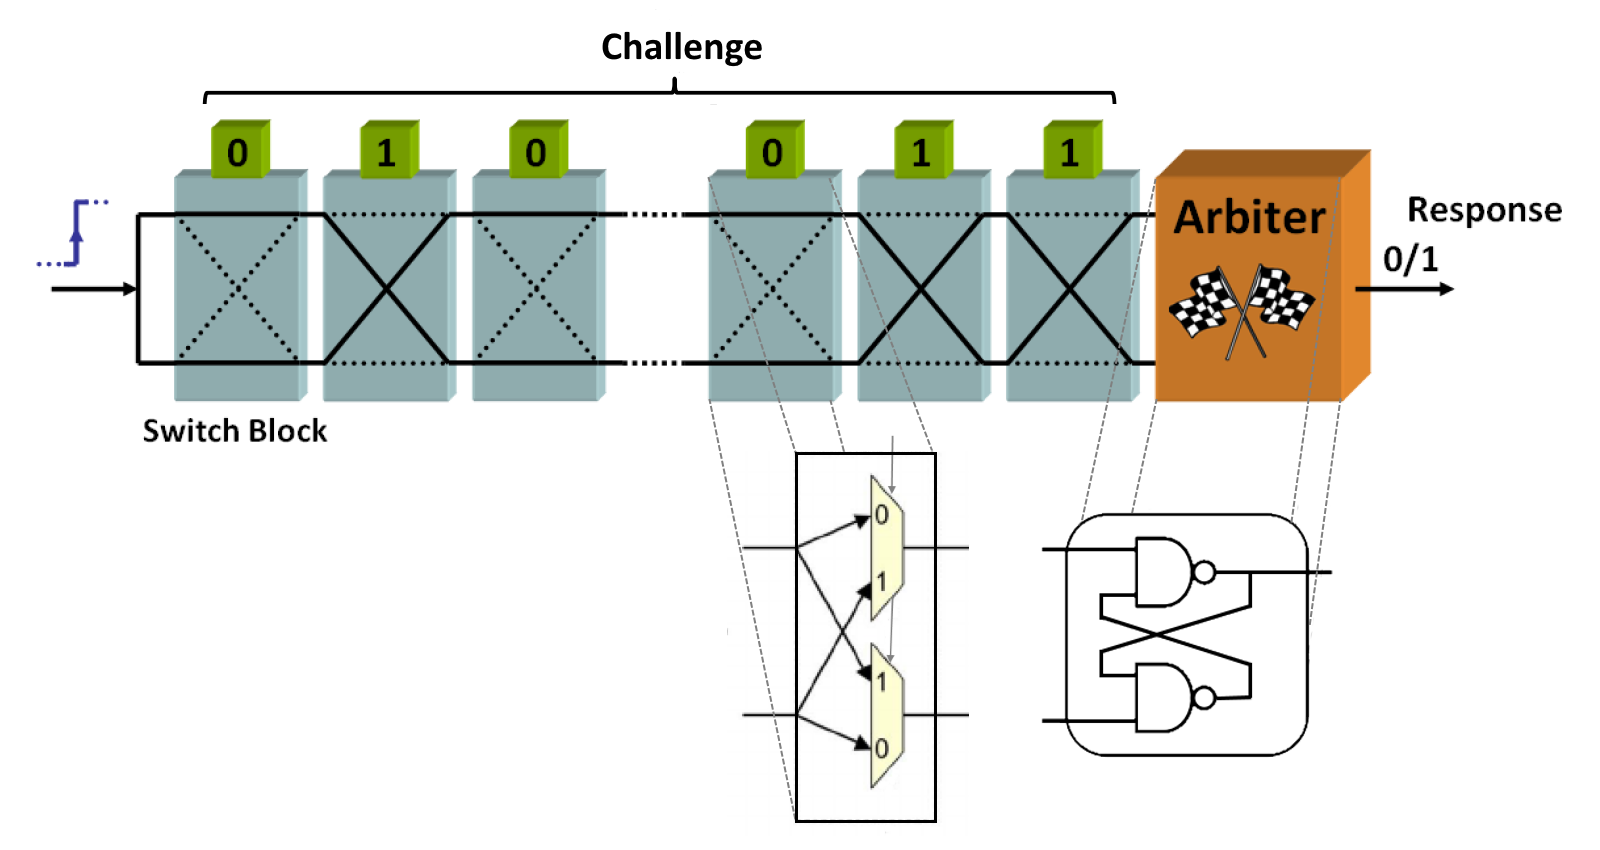
\includegraphics[width=0.9\textwidth]{images/arbiter_4.png}}
	\caption{Construction of a basic arbiter PUF, \emph{switching blocks} realized with muxes and a \emph{SR latch} realized with NAND gates, modified graphic based on [seb 34]}
	\label{img:1}
\end{figure}

\textbf{\emph{Security Issues:}}
Though the challenge set is large still the number of delay paramerters which effect the PUF response are linear in n, hence the 2$^n$ challenges cannot generate independant reponses. A certain model or mathematical clone can be build for a given arbiter PUF if adversary learns the underlying delay parameters. This clone can accurately forecast the PUF reponse rendering the arbiter PUF hackable in security applications scenarios. Machine learning techniques like artificial neural
networks (ANNs) and support-vector machines (SVMs) can be employed to implicitly learn the underlying delay parameters by observing the challenge response pairs.

\subsubsection{SRAM PUFs}
\label{srampufs}

Static Random-Access Memory (SRAM) is a digital memory technology based on bistable circuits. [seb 34 section 2.4.4.]. Refer to fig [ ] for details of an SRAM cell. It consists of six MOSFETs transistors, out of which four are contained in two invertors. Each invertor comprises of one p-MOS and one n-MOS MOSFET. As you can see from fig [ ] the invertors are cross-coupled at SRAMs cell core. In logic sense, the circuit has two stable states (bistable), each state represented by a binary
digit (0 or 1) that is stored in the cell. Two MOSFETs are used to read and write the cell contents. An SRAM cell is volatile and does not store its state on power-off.\\

There are three possible operating points, two are stable and one is metastable fig [ ]. The deviation from stable points is automatically restored to its original point due to the feedback from the circuit. Adversely any deviation from metastable point is amplified by the positive feedback from the circuit and cell moves to either of the stable points. After the supply voltage $V_{DD}$ comes up the cell shifts to one of the preferred stable points, which is determined by the difference in
strength (device mismatch) of the MOSFETs in the cross-coupled invertor circuit. Due to performance and efficiency reasons the invertors are designed to be perfectly in sync, the device mismatch is a result of the random process variations in the silicon production process. This random preferred intial operating point is unique a specfic cell. For small mismatch the preferred initial stable point is determined by sign of the mismatch, though voltage noise can render the cell to
power-up in a non-preferred state. Finally the cells with almost zero mismatch power-up in metastable state and shift to one of the stable points randomly.\\

Most SRAM cells have strongly preferred cell-specific initial state due to the magnitude of the process variations on the device mismatch, only a small number of the cells have weak preferred or no preferred state, hence a typical SRAM cell exhibits strong PUF behavior. These cells are arranged in a large array giving millions of reponse bits, challenge for this cell assembly is the address of the cell.\\

\subsubsection{Ring Oscillator PUF}

Proposed by Gassend et al. [ ] it is another type of delay-based intrinsic PUF. There are two parts to ring oscillator PUF, first is the ring oscillator and other is the frequency counter which are arranged is a configuration as shown in the fig. [ ] and connected to a response generating algorithm. Gassend et al. uses a variant of the switch block base delay line similar to arbiter PUF \ref{arbiterpuf} which is transformed in a oscillator with the help of a negative feedback.
An AND gate is added to turn off/on the oscillation, which is fed to a frequency counter that counts the number of oscillating cycles in a fixed time interval. A same setup for ring oscillator on another device with same implementation has different counter value because of the silicon process variations which forms the basis of the PUF reponse.\\

\begin{figure}
\centering
\fbox{ 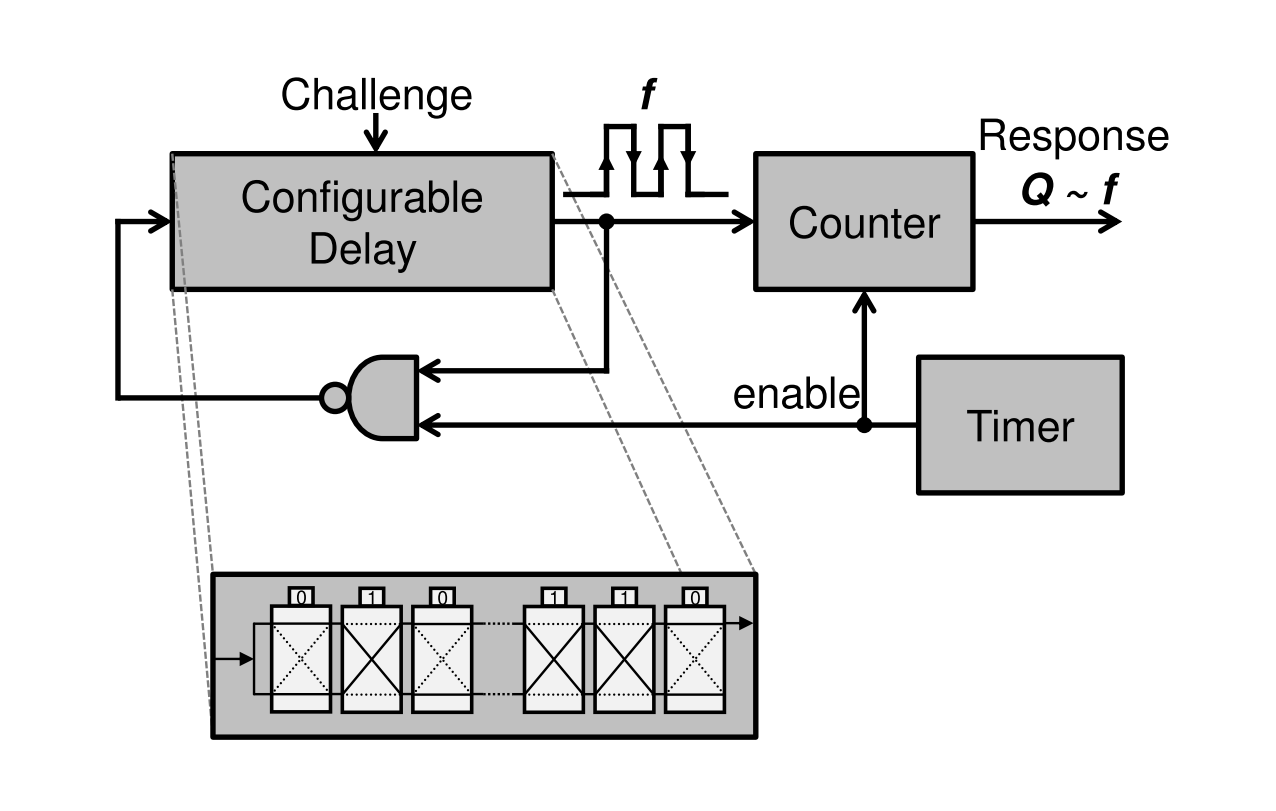
\includegraphics[width=0.9\textwidth]{images/ringPUF_1.png}}
\caption{Construction of a basic ring oscillator PUF, modified graphic based on [seb 34]} 
\label{img:2}
\end{figure}

There are some other side effects associated with ring oscillator PUFs, one of them is significant influence from the environmental conditions like temperature changes and voltage fluctuations. The frequency changes introduced by these factors outweigh the deviations caused by the process variations, so to counteract these changes we need a post processing technique known as \emph{compensated measuring}. The main idea is to calculate the ratio of the frequency of two ring oscillators
on the same device since they both are affected with identical environmental factors, hence the ratio would be more uniform. According to observations average intra-distance distance between evaluations is approximately less than the average inter-distance by 50\% [seb 34 section 2.4.2] 

\subsubsection{Optical PUFs}

Even before the introduction of PUFs an unclonable identification system based on random optical reflection patterns was proposed in [th 53 section 3.1.1]. Proposed by Pappu et al. as Physical one-way functions (POWF) optical PUF contains a microstructure constructed by blending microscopic (500 $\mu$m) refractive glass spheres in a miniature (10 x 10 x 2.54 $mm$) transparent epoxy plate. This token is illuminated with a helium neon laser which produces a irregular wavefront,
the cause for this irregularity is the multiple scattering of the laser by the refractive particles. Finally a CCD camera captures the speckle pattern and digitally processed by applying Gabor Hash to it as a feature extraction procedure. [th section 3.1.1] The final output is a string of bits that deviates significantly if the orientation of the laser beam is even minutely changed.\\

Challenge is made up from the exact positioning of the laser and the resulting Gabor hash of the emerged speckle pattern is considered as response. The operation and implemetation for optical PUF is shown in fig [ ]. Number of experiments were performed by [th 41 42] for testing the characterstics of the optical PUF and following summarizes their results. These values are taken from the [pappu et al. and th 42]. Total four optical tokens used with 576 individual challenges, for the
responses intra and inter distance measures were evaluated with average inter-distance of $\mu_{inter}$ = 49.79\% and average intra-distance of 
$\mu_{intra}$ = 25.25\%. One of the main limitation of such an optical PUF is the burdensome large setup consisting of a laser and mechanical positioning system. They are classified as Non-electronic, non-intrinisic and strong PUFs.\\

\begin{figure}
\centering
\fbox{ 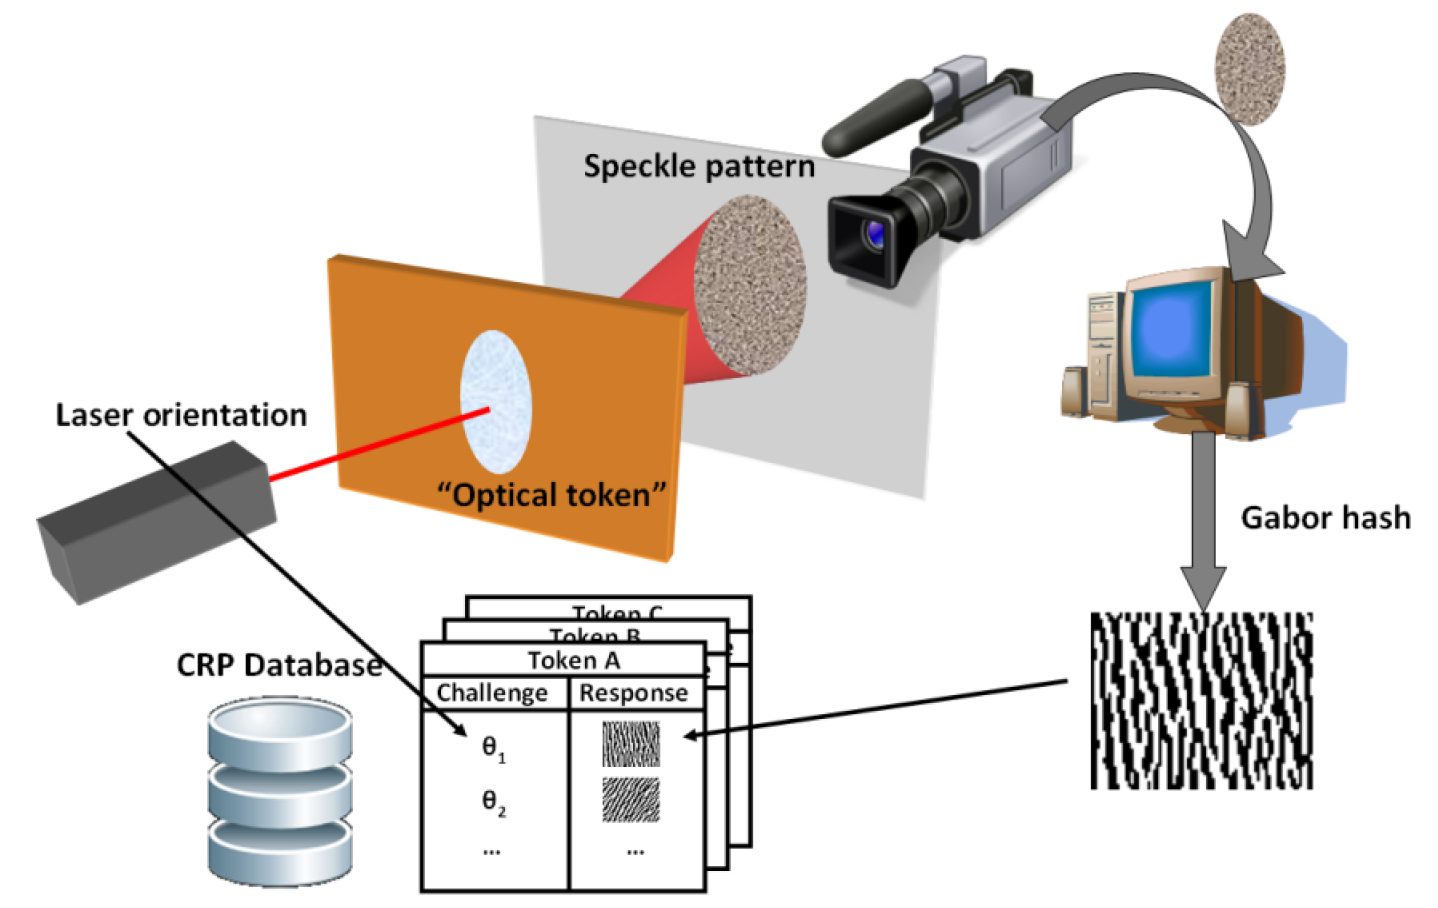
\includegraphics[width=0.9\textwidth]{images/opticalPUF.png}}
\caption{Construction of a basic optical PUF as proposed by Pappu et al. \cite{18,19}.}
\label{img:3}
\end{figure}

\section{linear codes, bch , golay}
In order to understand the working of the toolkit and fuzzy extractors (discussed later in section ) we need to look at the two specific type of linear codes. The following sections and subsections discuss the basics of linear codes and their mathematical constructs. After the intial explanation of what linear codes are, we go on to explain BCH codes and golay codes that are used in the PUF toolkit to extract private and public keys in conjugation with SRAM PUFs. The major
content for these sections is inspired from [ln, bf book chap 2].\\

Before diving into linear codes let us first look at the definition of Field from the book [chap 2]:\\
\textbf{Definition} A field F is given by a triple (S, +, ·), where S is the set of elements containing
special elements 0 and 1 and +, · are functions $F \times F \rightarrow F$ with the following properties:
\begin{itemize}
	\item Closure: For every a, b $\in$ S, we have both a + b $\in$ S and a · b $\in$ S.
	\item Associativity: + and · are associative, that is, for every a, b, c $\in$ S, a +(b +c) = (a +b)+c and a · (b · c) = (a · b) · c.
	\item Commutativity: + and · are commutative, that is, for every a, b $\in$ S, a + b = b + a and a · b = b · a.
	\item Distributivity: · distributes over +, that is for every a, b, c $\in$ S, a · (b + c) = a · b + a · c.
	\item Identity: For every a $\in$ S, a + 0 = a and a · 1 = a.
	\item Inverse: For every a $\in$ S, there exists its unique additive inverse -a such that a + (-a) = 0. Also for every a $\in S \backslash \left\{0\right\}$ there exists its unique multiplicative inverse $a^{-1}$ such that a · $a^{-1}$ = 1.
\end{itemize}

\textbf{Lemma} Let p be a prime. Then $F_p = (\left\{0, 1, . . . , p - 1\right\}, +_p , \cdot_p )$ is a field, where $+_p$ and $\cdot_p$ are
addition and multiplication mod p. [bf chap2]

example $F_2 = \left\{0,1\right\}$ is a binary finite field with two symbols 0 and 1 where + and $\cdot$ are operations modulo 2.

\textbf{Linear Subspaces},  before defining Codes and linear Codes we need to know what is a linear subspace.
\textbf{Definition} $ S \subseteq F_q^n $ is a linear if the following properties are satisfied:[bf chap2]
\begin{enumerate}
	\item For every $x,y \in S, x+y \in S$, where addition is vector addition over $F_q$
	\item For every $a \in F_q$ and $x \in S, a\cdot x\in S$, where multiplication is over $F_q$
\end{enumerate}

A simple example to understand above Definition and Lemma is $F_5^3$\\
S = \{(0, 0, 0), (1, 1, 1), (2, 2, 2), (3, 3, 3), (4, 4, 4)\}.
As you can see (1, 1, 1) + (3, 3, 3) = (4, 4, 4) $\in S$ and 2.(4, 4, 4) mod 5 = (3, 3, 3) $\in S$ as stated in the definition

Now, we can define a \textbf{linear Code} as a code of length n over the field F is a subspace of $F^n$ . The words of the codespace $F^n$ are vectors, and we often refer to codewords as codevectors.
If C is a linear code that, as a vector space over the field F , has dimension k,
then we say that C is an [n, k] linear code over F , or an [n, k] code [linear.pdf]. The \emph{distance} of the code is number of symbols changes required in a codeword to assume another codeword. eg. let C(3,3) is a subspace $F_2^3$ if two code words 000 and 111 , then distance between them is 3 since we need to change three symbols 0 to 1.
The \emph{rate} of an [n, k] linear code is \textbf{k/n}. If C has minimum distance d, then C is an [n, k, d] linear code over F .
The number n - k is called the \emph{redundancy} of C [linear.pdf]

This section tried to cover the basics for understanding BCH codes and Golay Codes, in no way we claim the completeness of the mathematical constructs and other proofs that are skipped. Please refer to the references for more details.\\


\section{Jaccard index}

\section{Congnicrypt Syonpsis}



%this chapter can be divided into 2 parts, implementation for PUF toolkit
% and integration into cogni UI
\chapter{Implementation}
\label{implementation}
%This chapter explains about the major tasks implemented in the thesis and new contributions made to the PUF Toolkit. The first part of the chapter briefly explains about the current PUF toolkit implementation, without delving much into the details. The second and more major part talks about the new modifications that were done to the toolkit in the form of BCH fuzzy extractor encoder and decoder integration, which were previously not a part of the main toolkit and presented as seperate executables
with seperate menu items. We then go on to explain the Golay code implementation both the decoder and encoder, and explain their integration in the toolkit as a distinct menu item. Then the other modifications like the addition of \emph{'offsets from begining and end', error codes} and other intricate code developement changes are presented together as one section.\\

%TODO: write about hamming distance and jaccardi's index

The final two sections deal with cognicrypt details and the Java Native Interface (JNI), they first touch upon the basics of JNI
wrapper and the functioning of JNI with shared libraries packaged as JAR files that are accesible to Java compiler as external library. Finally, we describe the clafer model of the cognicrypt and how it assists users and Java developers, without any previous knowledge about cryptography, to select a strong PUF based secure key evaluation algorithm based on the questions asked by the cognicrypt. In the end of this last section we also talk about the xsl model of the cognicrypt that builds on
the clafer model to generate a boilerplate java code to help the Java developer by presenting him/her with a sample usecase of the Java code implementation showing a usage of the PUF evaluation algorithms that is robust and flawless.\\

For the implementation, the ISO standardize programming language C++ was chosen. This selection was made based on the efficient and general purpose features provided by C++. Apart from the object oriented and generic programming features, C++ has a high abstraction level and the compilation and code development can be done on diverse systems. The implementations are dissociated from a specific hardware to support a wide range of systems and applications. This makes the toolkit easier
to extned and conform to a particular hardware for next iterations. The JNI framework support native calls and the wrapper is written in Java, for clafer model we use Java script and json files along with the .cfr clafer extension modelling language(refer to github page [ ] for details) and xsl model to generate sample Java boilerplate code is written in xsl.\\

\section{PUF Toolkit}
The current implementation of the PUF toolkit was done and presented in the thesis [sebastian Master Thesis]. The main aim of the toolkit is to evaluate various PUF repsonse based on well established metrics and thereby helping researchers and designers to gain useful insights into the properties and behaviour of PUF responses. The toolkit implements the following list of metrics: \pagebreak

\begin{itemize}
	\item (Shannon) Entropy
	\item Hamming Weight
	\item Intra-Hamming Distance
	\item Inter-Hamming Distance
	\item Min-entropy
	\item Median and average
\end{itemize}

These metrics are well explained in the Master thesis Sebastian [ ], so we take the liberty to not go into the detail of explaining each metric here again. It must also be noted that there are other metrics and definitions that use identical concepts and/or apply the metrics in a different way to generalize the coorelation between different PUF instances and their reponses. More exhaustive and comprehensive information related to these metrics and definitions for PUFs can be found in [seb 37, 53, 26, 5].\\

Apart from the above mentioned metrics implementation the PUF based secure key storage is implemented already, using BCH encoder and Decoder in two seperate executables. The structure and the User design used in these two executables is similar to the PUF toolkit and to avoid confusion we shall refer to them as \emph{PUF-BCH encoder} and \emph{PUF-BCH decoder}.\\

\subsection{User Design}

The notion behind the console user interface design by inspired from Nielsen and Molich's nine user interface design guidelines [seb 45]. These guidelines and their resulting effects are shown the table \ref{tab:guidline_design} below:

\begin{table}[!ht]
\begin{center}
\begin{tabular}{cll}
\toprule
\multicolumn{1}{c}{\textbf{No.}} &\multicolumn{1}{c}{\textbf{Guideline}} & \multicolumn{1}{c}{\textbf{Effect}}\\
\midrule
\hline
1 & Simple and natural dialogue & Clear and logical dialogue structure\\

2 & Speak the user’s language & Clear instructions\\

3 & Minimize the user’s memory load & Clean design, brief help and guide texts\\

4 & Be consistent & Consistent design in all menus\\

5 & Provide feedback & Provide feedback and status\\

6 & Provide clearly marked exits & Provide ``back’’ and ``exit’’ in each menu\\

7 & Provide shortcuts & Inputs by abbreviations \\

8 & Good error messages & Provide useful error messages\\

9 & Prevent errors & Handle wrong inputs \\
\hline
\addlinespace
\bottomrule
\end{tabular}
\end{center}
\caption{The nine design guidelines according to [seb 45] and the effect on the UI design.}
\label{tab:guidline_design}
\end{table}

The design of the menu and the (sub-) menus is consistent and recurses itself to make the user interface more intuitive and friendly. Each menu option is written in clear and easy to understand instructions and the menu items are precisely structured to help the user navigate the toolkit with ease. The organization of the menu follows a hierarchical design and a ``back'' function is provided for the user to go to the parent menu. A conceptual depiction of the User Interface is shown in Figure
\ref{img:gui_design}. The Graphical User Interface (GUI) is subdivided into four parts, the color markers are related to the illustration in \ref{img:gui_design}.

\begin{itemize}
	\item The first part, marked in yellow, is the \emph{header}. It gives the user general information, like the title of the current (sub-) menu or brief instructions.
	\item The second part of the gui shows the options and functions that the user can choose from the (sub-) menu, the number infront must be input by the user in the last part of the GUI. The conceptual illustration for the part is marked in red and is called as \emph{Menu}.
	\item Below the Menu part there is \emph{settings and results} that are marked in blue. It shows the current configuration and provides the user with essential information that is vital for the actual computation of the main function. It also shows the output after the computation is performed in the result part of this section.
	\item The fourth part of the GUI is for \emph{feedback} and inputs and is marked in green. It presents the user with the actual processing status, or if an error occurred and the type of the error. Also, it contains a user interactive input cursor, a number must be typed in by the user in order to select the options/functions from the second part, Menu of the GUI.
\end{itemize}

\begin{figure}
\centering
\fbox{ 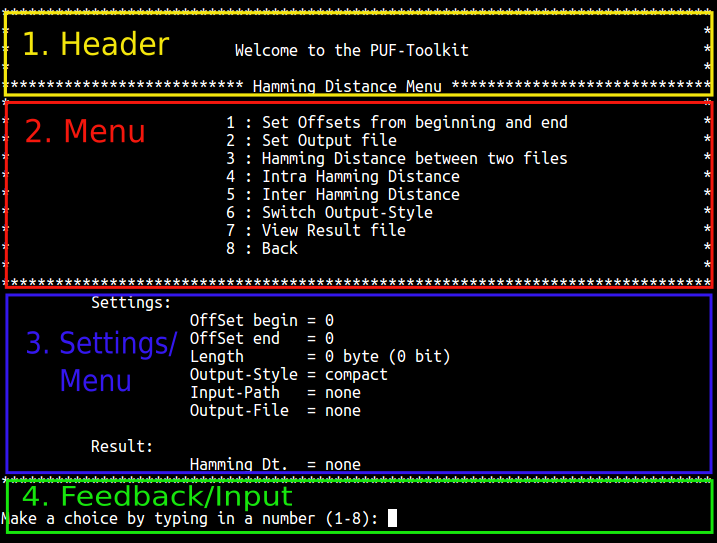
\includegraphics[width=0.9\textwidth]{images/toolkit_gui4.png}}
\caption{Conceptual design of the PUF Toolkit user interface.}
\label{img:gui_design}
\end{figure}

The design of the GUI is kept simple without the use of extended graphic components to keep the toolkit compatible with other operating systems like linux. The UI shows only relevant information depending on the current state of the program and potrays a simple but aesthetic clean design. Error correction and incorrect user input is efficiently handled, all possibile inputs are exhausted and depeding on the false input, meaningful errors information is displayed to the user, that can be used to
recover from the erroneous state. Also for all mandatory inputs a brief guide / help text with examples is shown, the current settings are saved and kept in each (sub-) menu (wherever applicable) to avoid unecessary redudant input.\\

Rigorously complying to the standardized design guidelines for the toolkit, resulted in a effective and intuitive console user interface.
This in turn decisively supports developers and researchers in the PUFs reponses evaluation.[seb thesis]

\begin{figure}
\centering
\fbox{ \includegraphics[width=0.97\textwidth]{images/PUF_Toolkit.pdf}}
\caption{Heirarchical Structure of the PUF Toolkit menu and available options}
\label{img:puf_menu}
\end{figure}

\section{Hamming Distance Menu}
\label{Hamming_Distance_menu}
The hamming distance functionality was added to and integrated as part of this Master thesis. Hamming Distance between two bit strings of same length is defined as the number of the bits that differ amongst the two binary bit strings. For eg. if we have two string \emph{A = 1100} and \emph{B = 1010} then the hamming distance between them would be ``\emph{two}'', since the bits at second and third position (starting from the left) differ between these two strings. The implementation of
this functionlality is straightforward, using the in-built \emph{bitwise XOR} operation of the ISO C++ standard and then counting the number of ones in the resulting string, which is nothing but calling the hamming distance function on the resultant string.\\

As depicted in the figure \ref{img:gui_design} above there are other options like \emph{Intra Hamming Distance} and \emph{Inter Hamming Distance} in the Hamming Distance Menu, that are organized later as subsections where we explain about the different modes and other options and plausible input values the user can select from them. For now we direct our attention at the other menu items.\\

The first menu item is related to the \emph{\textbf{Offsets}} that are mandatory for the user to input and the first query that must be answered after the toolkit is run. Since the PUF toolkit is designed for evalutation of PUF responses that are in binary format and not all the data in PUF reponse binary file is useful for evaluation the user can manually select how much he/she desires to skip the data (in bytes) from the beginning and the end of the file using this \emph{Offsets} option.
For example the first $400$ bytes of the PUF response of a (TI) Stellaris LM4F120XL Launchpad Evaluation Kit are used during the booting process and are not random, so they are irrelevant in PUF responses evaluation. These kind of device specfic behavior requires suitable handling to ensure valid results.\\

Consequently the \emph{Offset} determines the selection range of the bytes from the PUF response for calculation and also establishing the actual \emph{length} of the response. For eg. if a PUF response is 32784 bytes long and we skip 400 from the beginning and 200 from the end, the actual length becomes $32784-600 = 32184$ bytes and the processing starts from the $401^{th}$ byte till $32184^{th}$ byte.\\

The result of the Hamming Distance between two PUF responses can be optionally stored in an output file that is set using the option \emph{two}. This is not mandatory if we are evaluating only two files but in cases of Inter/Intra Hamming distance this option becomes mandatory. Another functionality added to the Hamming Distance and other Functions in the toolkit as well is that of the Fractional Distance. \newline
$\S$\emph{Defintion}: We define \emph{Fractional Hamming Distance} as the Hamming Distance between two PUF
responses divided by their length. For example if Hamming Distance between two PUF responses each of length 31784 bytes is 10, then their Fractional Hamming Distance would be $ 10 / 31784 = 0.000314624$ (NOTE: the toolkit displays the fractional hamming distance rounded off to 9 digits after decimal).\\

The Hamming Distance can be calculated using option \emph{three} that will ask for the two PUF responses binary filenames and if the path and filenames are correct, the results will be displayed in the fourth part of the GUI. If the output filename was given before then the result is also stored in that file and can be viewed using the option \emph{seven}.\\

In order to understand the code flow and working of the hamming distance function it is vital to look at the structure \emph{Item} and its data members. This structure is used by other menus in the toolkit to share the current settings and global configurations like Offsets, filenames, paths etc. and thereby reducing the user's effort and memory load. The table \ref{table:item} only highlights the data members and their purpose that are relevant to Hamming Distance Menu. The other data members
for the time being are not shown and will be discussed in relevant sections.\\

\begin{table}[!ht]
	\begin{center}
		\begin{tabular}{ll}
			\toprule
			\multicolumn{1}{c}{\textbf{struct \emph{Item}}} & \multicolumn{1}{c}{\textbf{Purpose}}\\
			\midrule
			\hline

			\emph{offset\_begin} & Defines the starting point in a binary file (bytes to skip from beginning)\\

			\emph{offset\_end} & Defines the ending point in a binary file (bytes to skip from end)\\

			\emph{input\_length} & Defines the number of bytes to use \\

			\emph{input\_file\_name} & Defines the name of the first input file (name and path)\\

			\emph{input\_PUF\_name} & Defines the name of the second input file (name and path)\\

			\emph{output\_file\_name} & Defines the name of the output result file (name and path)\\

			\emph{zeros} & Stores the occurrences of 0s in a defined file\\

			\emph{ones} & Stores the occurrences of 1s in a defined file\\

			\emph{frd} & Stores the fractional distance in a defined file\\

			\emph{result} & Stores the result and feedback regarding the calculations\\

			\emph{HD\_error\_pos} & Additional error information \\

			\hline
			\addlinespace
			\bottomrule
		\end{tabular}
	\end{center}
	\caption{Definition of the elements of the data structure \emph{Item} and their purpose.}
	\label{table:item}
\end{table}

The four lines of code form the basic building block for hamming distance as shown in the listing \ref{lst:hammingdt}. First the data is read from the two input PUF files into two arrays of size \emph{dsize} where dsize is equal to the length of the files after applying the Offsets, then as depicted in lines 3-5 of the listing \ref{lst:hammingdt} each byte of the data are bitwise XORed and the result in stored in a third array of same length. So the resultant data array contains
\emph{ones} in the position where bits differ in the two PUF responses. We then just need to count the number of ones in the XORed result.
This is done by calling the function \emph{hammingwt} abbreviated in the code for Hamming Weight.\\

\begin{center}
\begin{minipage}{0.7\textwidth}
\begin{lstlisting}[frame=single,language=C++,
commentstyle=\color{green},
backgroundcolor=\color{gray},
keywordstyle=\color{blue},
stringstyle=\color{orange},
basicstyle = \ttfamily \color{black} \footnotesize,
caption={Hamming Distance calculation using hamming weight and bitwise XOR operator} ,
label={lst:hammingdt},
captionpos=b,
numbers=left]
    //bitwise XOR f1data and f2data
    //to get the positions where bits differ
    for (i = 0; i < dsize; i++) {
        data[i] = f1data[i] ^ f2data[i];
    }
    //calculate hamming distance
    item->ones = hammingwt(data, dsize);
    item->frd = (float) item->ones / dsize;
\end{lstlisting}
\end{minipage}
\end{center}

Hamming Weight is one of the essential function of the toolkit and it is also referred to by other functions its important that we list its code here. Listing \ref{lst:hammingwt} shows the Hamming Weight function as implemented in the toolkit, it takes the data array as a character pointer and its size as arguments. The for loop in lines 5-14 takes each byte of the data and then bitwise ANDs with each bit position (total 8 bit-positions) to count the total occurences of ones in the byte. This process is
iterated for the entire length ``size'' of the array, each time incrementing the counter ``wt'' whenever a one is encountered and finally the hamming weight is returned to the caller function.\\


\begin{center}
\begin{minipage}{0.7\textwidth}
\begin{lstlisting}[frame=single,language=C++,
commentstyle=\color{green},
backgroundcolor=\color{gray},
keywordstyle=\color{blue},
stringstyle=\color{orange},
basicstyle = \ttfamily \color{black} \footnotesize,
caption={Hamming Weight calculation using bitwise AND operator} ,
label={lst:hammingwt},
captionpos=b,
numbers=left]
int hammingwt(char *data, int size)
{
    int i;
    int wt = 0;
    for (i = 0; i < size; i++) {
        (data[i] & 0x80 ? wt++ : wt); //8th bit position
        (data[i] & 0x40 ? wt++ : wt); //7th bit position
        (data[i] & 0x20 ? wt++ : wt); //6th bit position
        (data[i] & 0x10 ? wt++ : wt); //5th bit position
        (data[i] & 0x08 ? wt++ : wt); //4th bit position
        (data[i] & 0x04 ? wt++ : wt); //3th bit position
        (data[i] & 0x02 ? wt++ : wt); //2nd bit position
        (data[i] & 0x01 ? wt++ : wt); //1st bit position
    }
    return wt;
}
\end{lstlisting}
\end{minipage}
\end{center}

\subsection{Intra-Hamming Distance}
\label{intra_hd_section}
This section explains the Intra-Hamming Distance feature which is comparison of the PUF responses from the same device. As discussed in section \ref{intra_inter_section} we already observed that the PUF responses from the same device are not identical due various factors like voltage fluctuation,  temperature variation and other aging effects, which gives rise to Intra distance within the responses. ``Intra'' means on the inside, so we evaluate the PUF instance from within by assessing the Hamming Distance within
these responses. Since the hardware from which the SRAM PUFs are obtained are kept in a single directory, we need only to give the ``input path'' for processing Intra Hamming Distance, the output file option is mandatory to process Intra HD because the results must be stored for all the responses in a file to be viewed later. Alongwith the Hamming Distance between PUF responses the fractional distance is also saved for better assessment of the PUF instance.\\

A crucial attribute in the ``Switch output-style'' which can be used to change the save format of the output file, there are two possibilities for Intra HD: \emph{compact} and \emph{minimal}. The compact mode takes each file in the directory and recursively compares with all the other files, then the second file is chosen and compared with the all the other except the first one and so on. The fig. \ref{img:4_intra_WP} illustrates this comparison.  The output style ``\emph{compact}'' is the default format style and should be used
as an output format for a regular text file. Due to the symmetrical behaviour of the comparison ( A to B = B to A) we need not exhaust all 1-to-1 possible combinations. So in compact mode first entry from the directory is compared to all the other till last entry, then the second entry is compared to the third entry till last file, then the third with fourth entry and so on till we are at the last file which need not be compared to any of the above entries since we have already exhausted the
symmetric comparisons.\\

\begin{figure}
\centering
\fbox{ 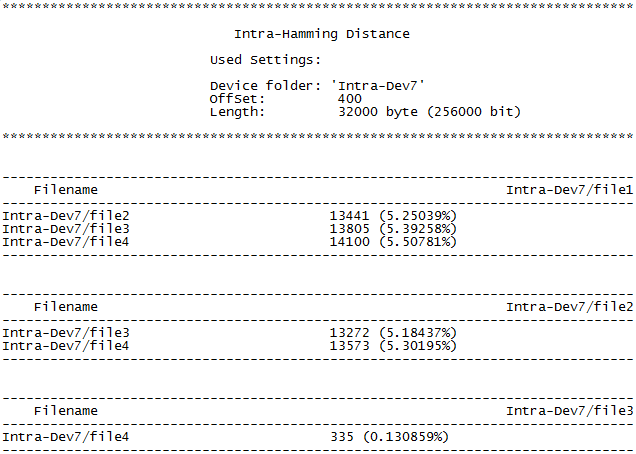
\includegraphics[width=0.9\textwidth]{images/4_intra_compact.png}}
\caption{Visualization of the \emph{compact} output style format.}
\label{img:4_intra_compact}
\end{figure}

\begin{figure}
\centering
\fbox{ 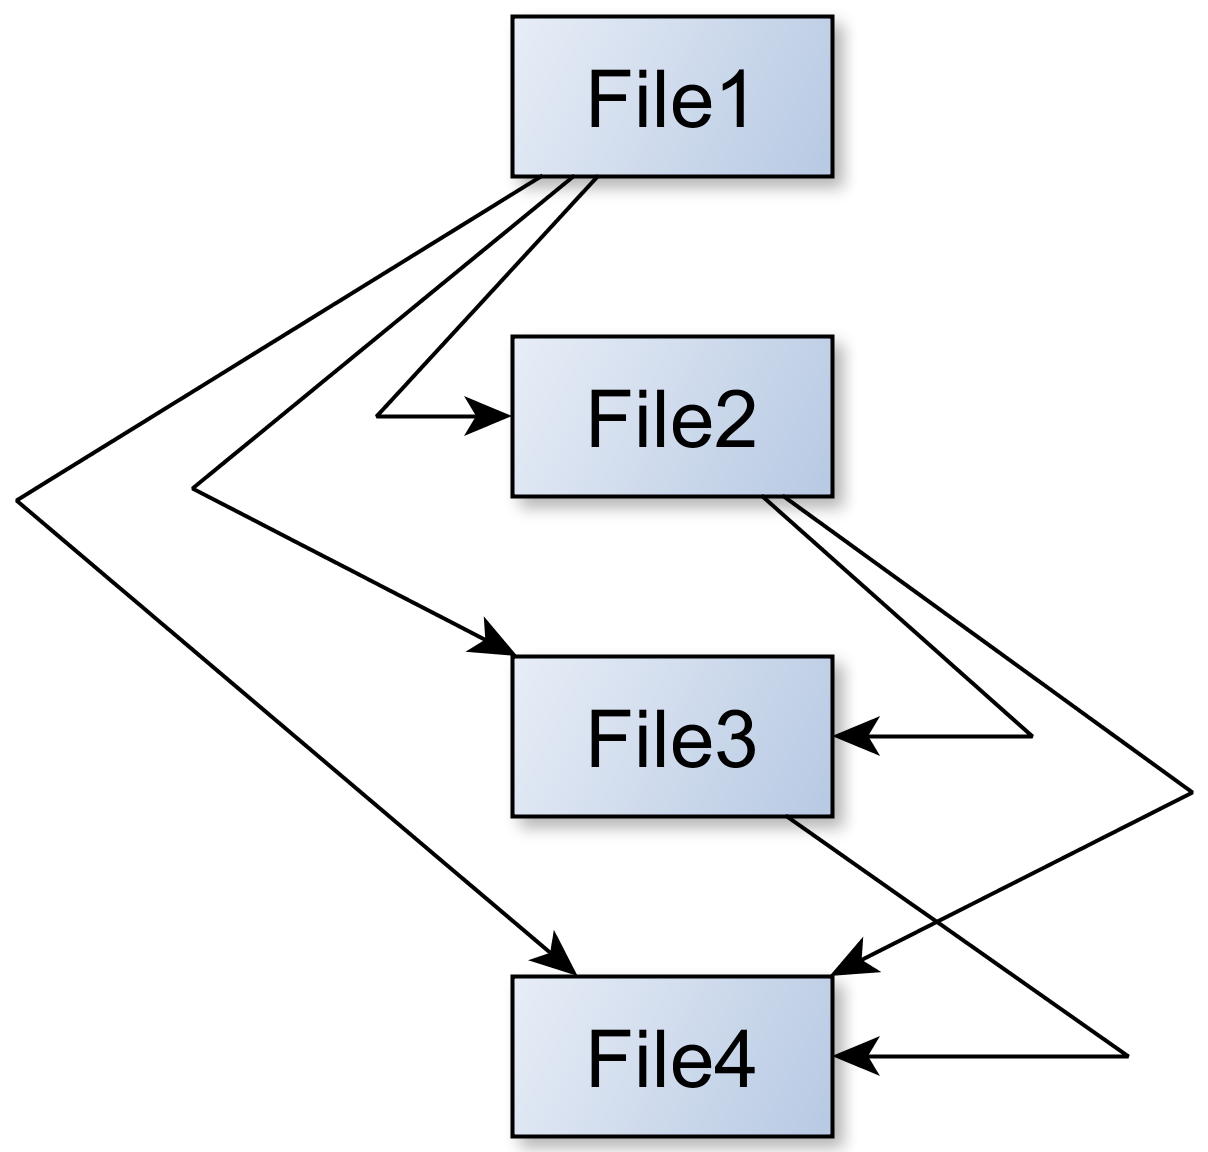
\includegraphics[width=0.4\textwidth]{images/Intra.png}}
\caption{Exemplary illustration of the working principle of the \emph{compact} mode, for the intra-Hamming distance.}
\label{img:4_intra_WP}
\end{figure}

A sample output file with compact style format is shown in Figure \ref{img:4_intra_compact} that evaluates the PUF instance from a single directory using Intra Hamming Distance metric, it also appends the fractional distance information to the file. It consists of a header with general information that shows the configuration (like offsets, device folder etc.) that was used for evaluation and three tables. In the upper right corner of each table the utilized input file is shown and on the left side of the table
the files, that are compared to the selected input file, are displayed. The Hamming Distance and Fractional Hamming Distance, seperated by a tab length are printed in the center (right) of each table. The
\emph{minimal} output style strips off all the path and filename info and only saves the Hamming Distance values seperated by spaces, this type of file format can be used by another metric of the toolkit called Median and Average [seb thesis section median] calculation which accepts only files containing plain numbers seperated with space. The \emph{View} option can be used to look at the output/result file.\\

\subsection{Inter Hamming Distance}
\label{inter_hd_section}
Contrary to the comparisons between PUF responses from the same device, Inter Hamming distance evaluates responses from different PUF instance. The co-relation is again based on the same metric Hamming Distance. In this case the toolkit can simulatneously compare from 2 to 99 PUF instances. All the PUF responses from a specific instance are arranged in a single directory so that means the toolkit can take input paths between 2 and 99 to evaluate different PUF devices. The output
style in addition to compact and minimal has a \emph{detailed} as an alternative. The compact and minimal style formats are same as Intra Hamming Distance, but the detailed style differs from the compact style that it does not implicitly ignores the duplicate symmetric comparisons and therefore maps out all the permutations and combinations between files of different folders. It should be noted that Inter Hamming Distance metric does not compare PUF responses in the same directory. So
in detailed mode, the first directory all the responses are compared to all the PUF responses from the remaining 3 to 99, then all files in second folder are compared to all the files in all the other folders except its own, and so on. The Figure \ref{img:inter_output} shows a sample output with 3 input paths, for compact mode we need to ignore the duplicate comparisons so we take the following approach:
\begin{itemize}
	\item store all the filenames and their corresponding paths from all but last folder in list1.
	\item store all the filenames and their corresponding paths from all but first folder in list2.
	\item iterate over list1 (iteration 1-4) and compare the list1 objects with all entries of list2.
	\item remove the second folder objects from list2.
	\item iterate over list1 (iteration 5-7) and compare the list1 objects with all files of list2.
\end{itemize}

\begin{figure}
\centering
\fbox{ 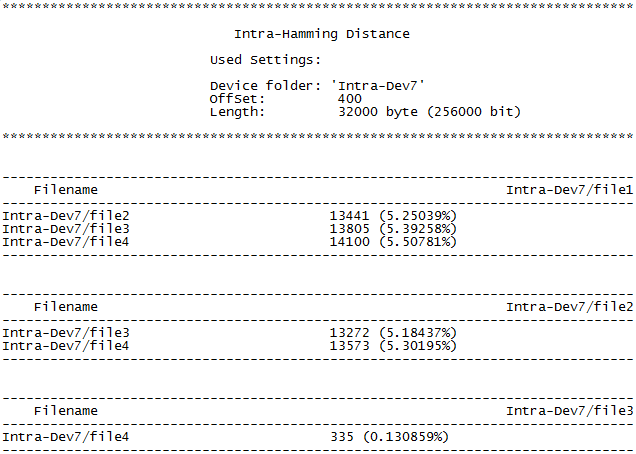
\includegraphics[width=0.4\textwidth]{images/4_intra_compact.png}}
\caption{A sample output showing the visualization of the inter hamming distance \emph{compact} output style format.}
\label{img:inter_output}
\end{figure}

\begin{figure}
\centering
\fbox{ 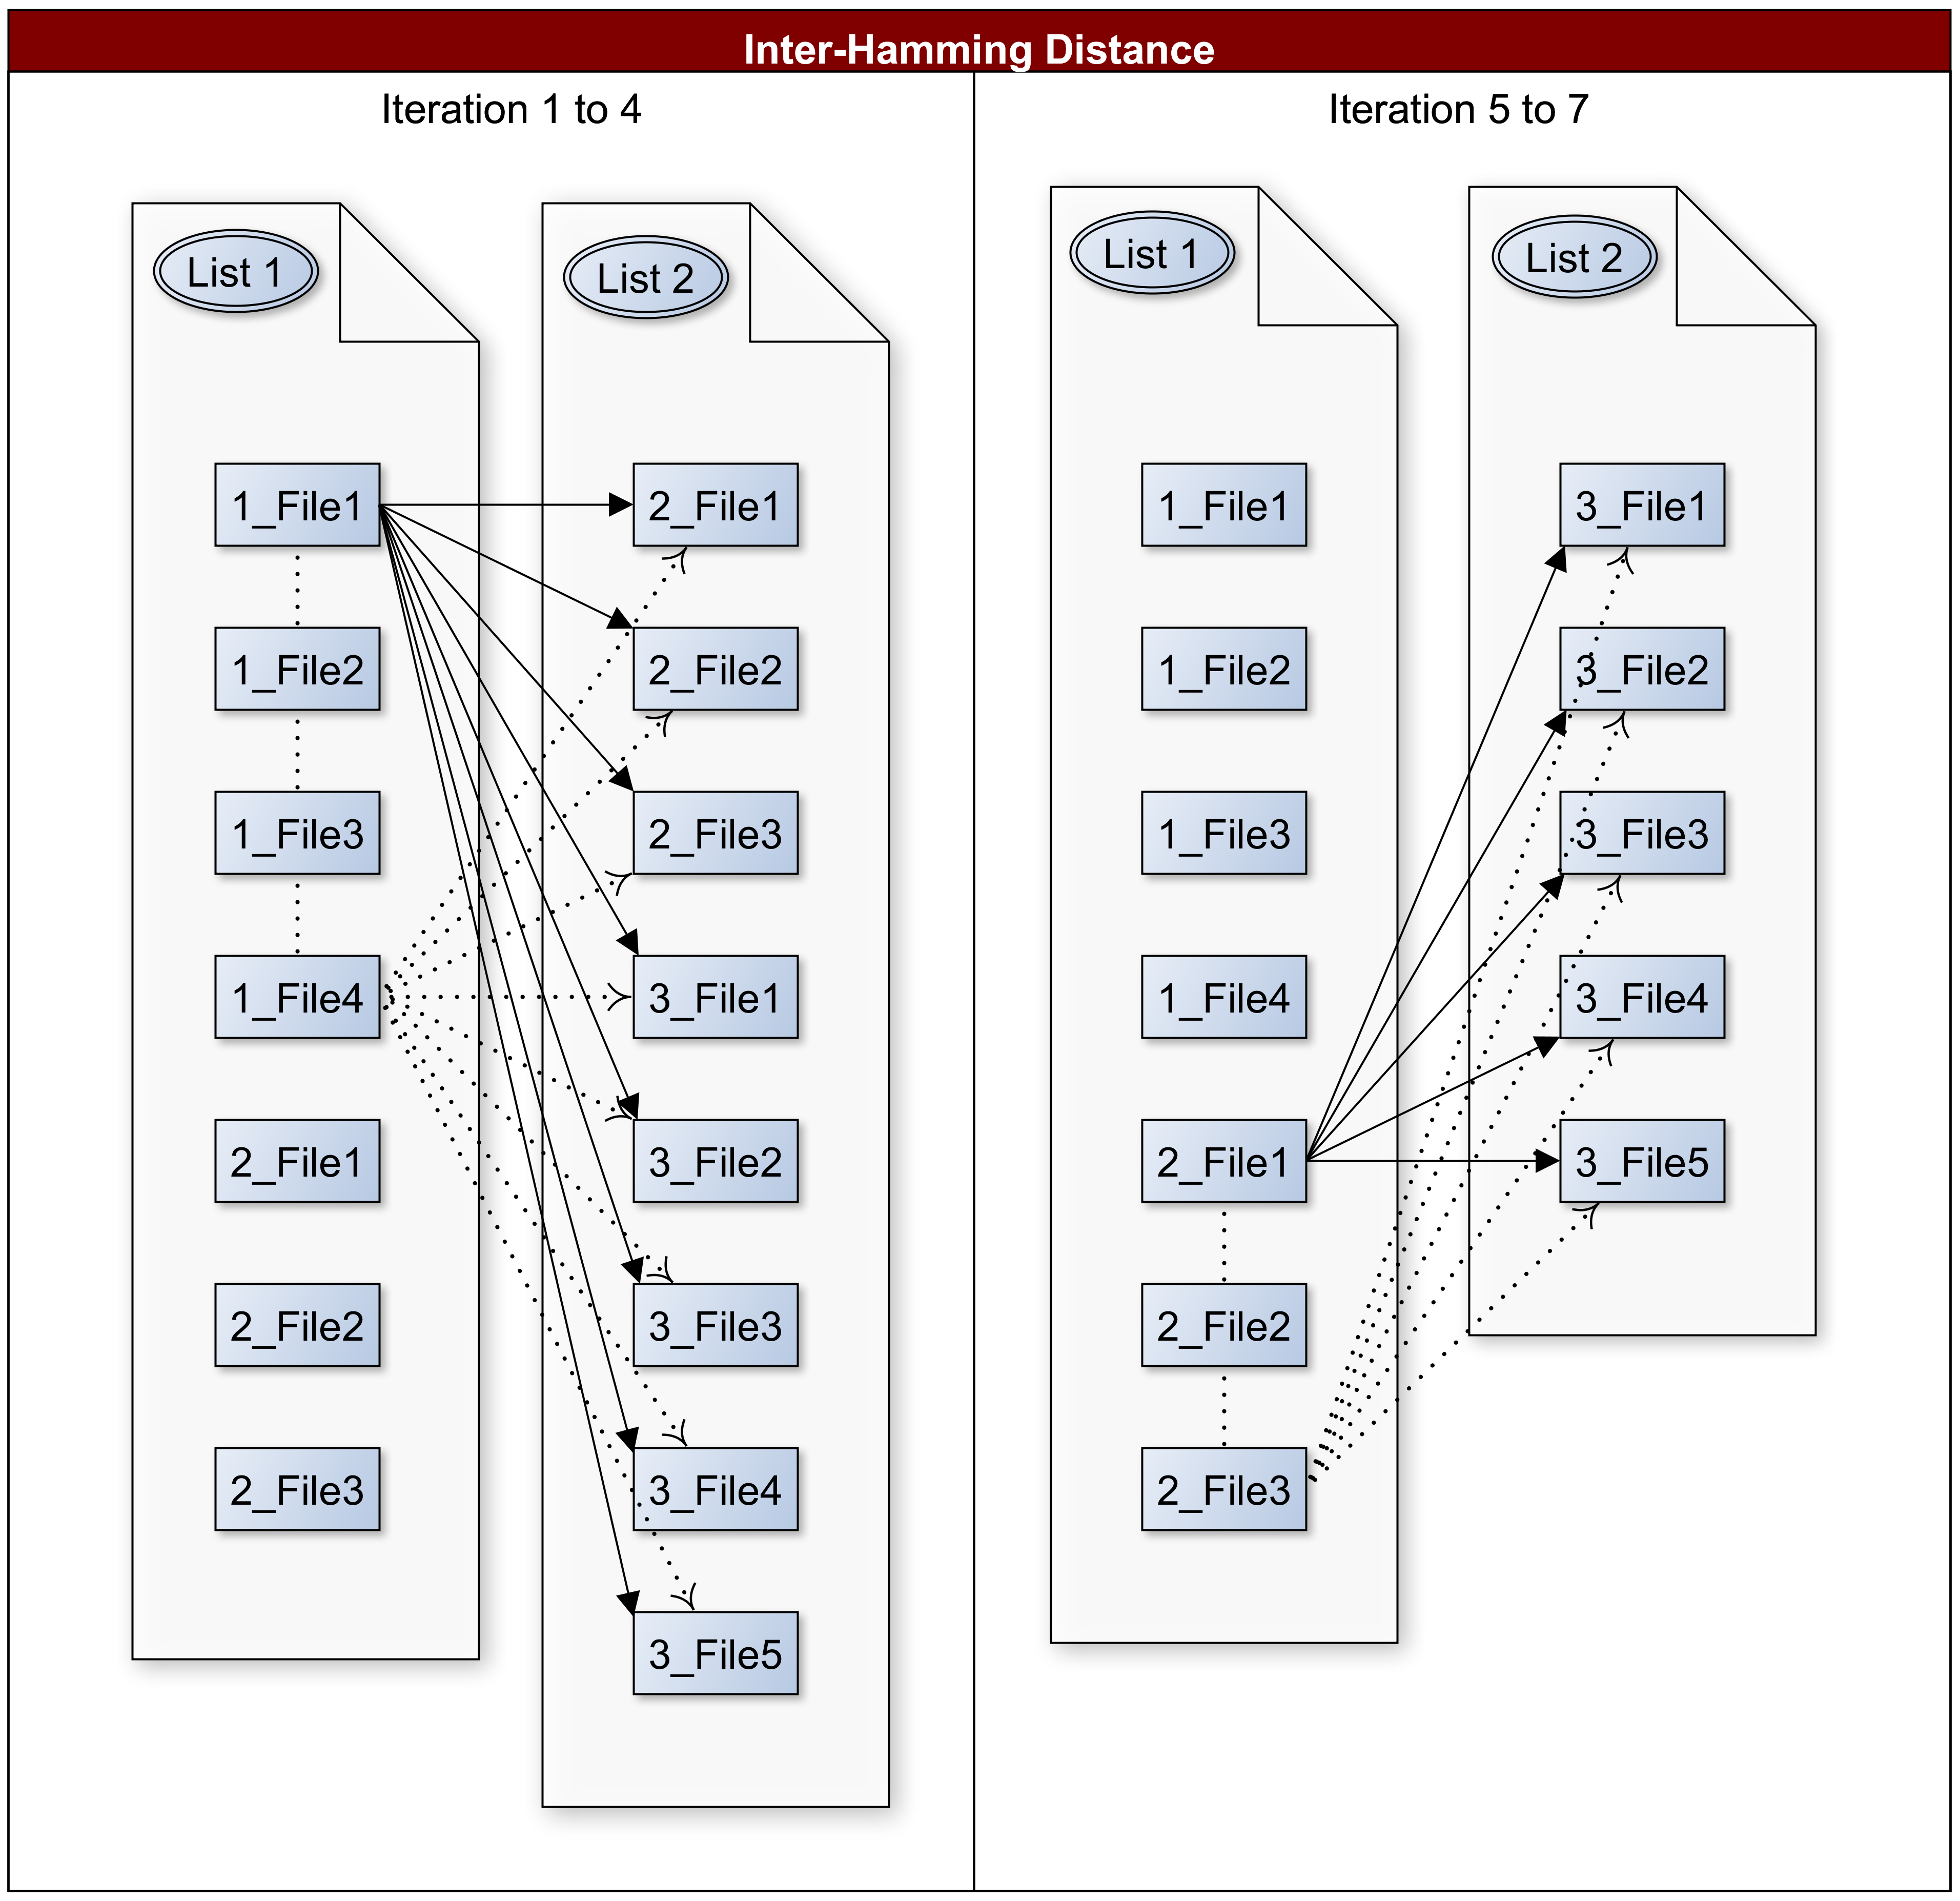
\includegraphics[width=0.4\textwidth]{images/Inter_itr.png}}
\caption{Exemplary illustration of the working principle of the \emph{compact} mode, for the intra-Hamming distance.}
\label{img:inter_compact}
\end{figure}

This process is summarized in Figure \ref{img:inter_compact} for three folder input and is generalized for more inputs. We emphasize on the inner workings of the modes because the exact same techniques are used for Jaccardi's index that will be discussed later in this chapter.\\

\emph{Menu Modifications:} In contrast to the original toolkit where Intra and Inter Hamming Distance were seperated in their own sub-menus, the new changes merges both of them under Hamming Distance Menu. Seeing as it is relevant to combine them if they use the same underlying metric, on the other hand the Hamming Weight menu item was untouched since it takes only one PUF response file as an input and gives out its hamming weight and there is no evaluation between two or
more files.\\


\section{Fuzzy extractor}
As discussed in section \ref{fuzzy_section} the PUF based secure key storage uses Fuzzy Extractor technique that is divided in three phases \emph{(i)Pre-evaluation}, \emph{(ii) Enrollment} and \emph{(iii) Reconstruction}. We discuss only the later two phases, where these two phases follow a seperate implementation of the respective dedicated functionalities, according to [seb 56]. The enrollment phase employs Pis presented with the help of an entity relation diagram. Similar to BCH encoder
section we examine the changes required during merging with the toolkit in the subsection ``Integration Changes'' and finally talk about the verification steps taken to assert the correctness of the merged decoder functionality in the toolkit.\\UF BCH encoder which will be discussed first followed by the Reconstruction phase, that is
realized by the PUF BCH Decoder implementation. We will not go into the details of the actual implementation of the encoder and decoder since thay are already well documented in [Master theses sebastian], but rather explain the changes made to integrate these functionalities in the PUF toolkit.\\

The concept of fuzzy extractor in combination with BCH coding with linear repetition code and majority vote is depicted in Figures \ref{img:4_BCH_concept}, \ref{img:4_LR_HD} and \ref{img:4_MV_codewords}.\pagebreak

\begin{figure}[h]
\centering
\fbox{ 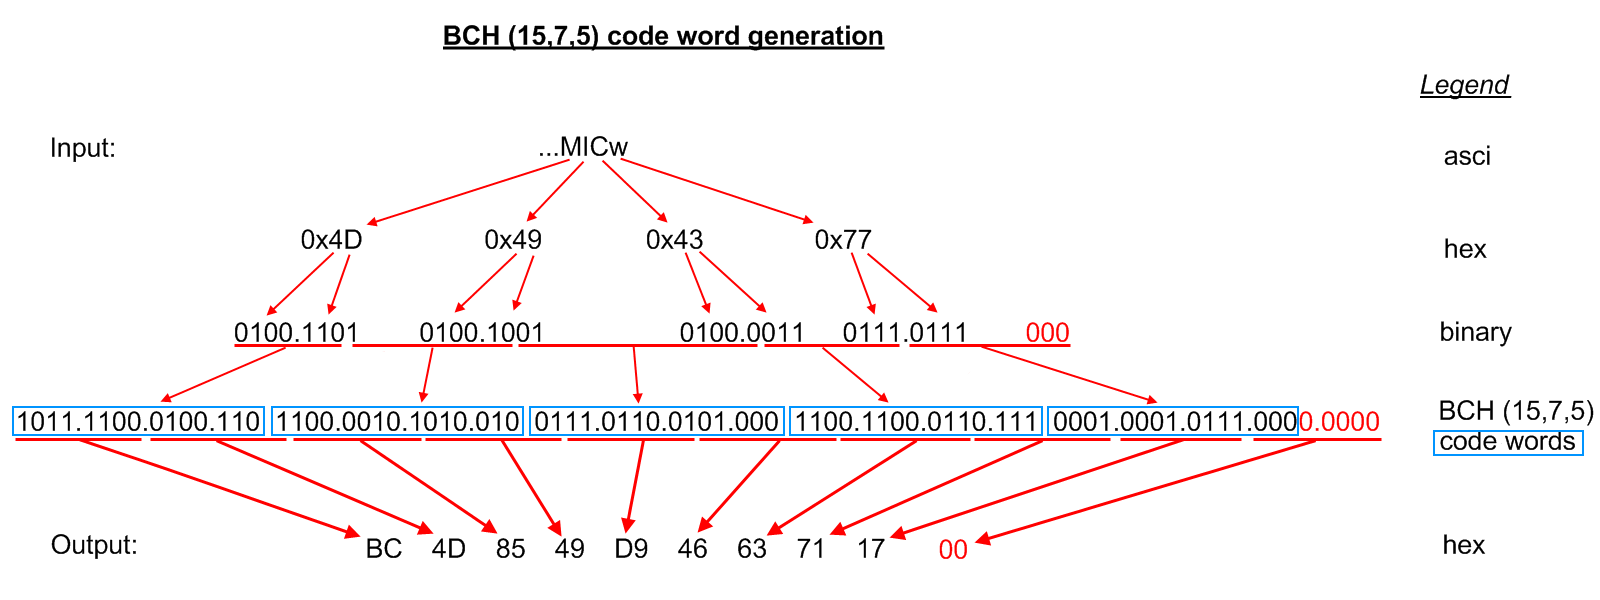
\includegraphics[width=0.97\textwidth]{images/BCHconcept.png}}
\caption{Exemplary code word generation with a BCH (15,7,5) code, based on \cite{10}.}
\label{img:4_BCH_concept}
\end{figure}

\begin{figure}[h]
\centering
\fbox{ 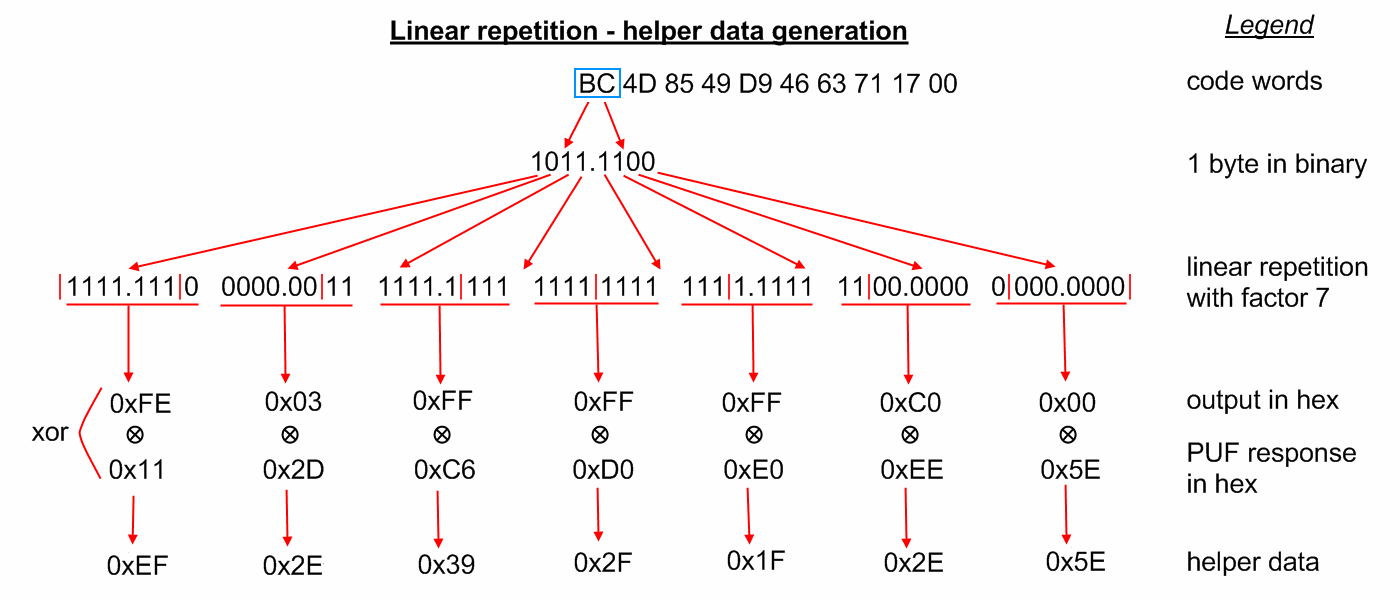
\includegraphics[width=0.97\textwidth]{images/LRhd.png}}
\caption{Exemplary helper data generation with a linear repetition code and factor 7, based on \cite{10}.}
\label{img:4_LR_HD}
\end{figure}

\begin{figure}[h]
\centering
\fbox{ 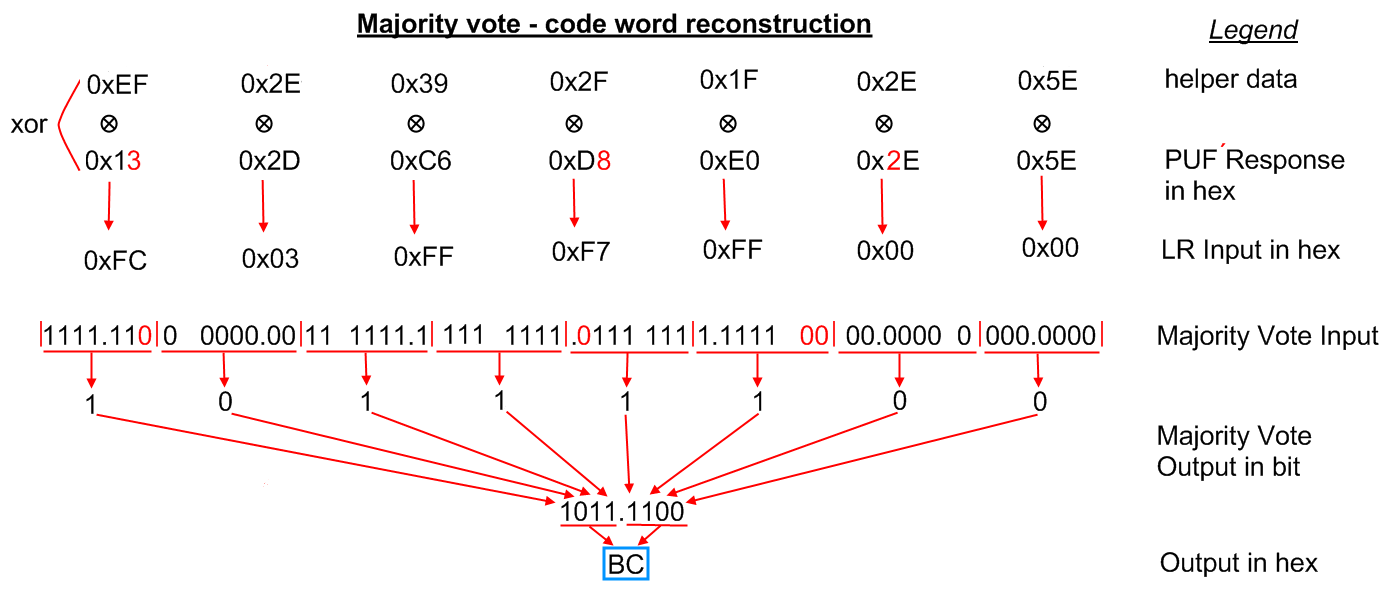
\includegraphics[width=0.97\textwidth]{images/MVrecon.png}}
\caption{Exemplary code word reconstruction with the majority vote and factor 7, based on \cite{10}.}
\label{img:4_MV_codewords}
\end{figure}

\subsection{PUF BCH Encoder}
This section first briefly mentions the implementation algorithm used in the BCH encoding of the data, after that the user interface is illustrated followed by a Entity relation diagram that shows major functions of the encoder. The changes are presented as a subsection named integration changes and the section is concluded by showing the steps taken to verify the integrated BCH encoder.\\

The BCH encoding implementation is taken from \emph{Morelos-Zaragozas Encoder/Decoder} for binary BCH codes in C [seb 43]. This algorithm uses systematic encoding to encode the message, hence the encoded codewords contain initial message in it, which is stripped from the codeword to get the helper data, using the BCH(n,k,d) (refer section \ref{bch_section}) the codewords are combined in groups of \emph{length k} and extra 0s are added to complete the last set . In the
second part of the enrollment of the fuzzy extractor the LR code is applied to the generated codeword, based on the user input the bits are repeated either 7 or 15 times, the Figure \ref{img:4_LR_HD} shows this LR process with factor 7. It was noted that there were some limitations to the original algorithm and the encoding only works for small values of $m$, after code review and research the error states were removed and/or documented.\\

Due to above mentioned limitations, the correct combination of BCH encoding and linear repetition code requires correct handling of the bounds. The length of the secret key in bits is denoted by $N$, to process the entire file with BCH (n,k,d) code we need \emph{len} iterations of encoding, this is defined in equation \ref{4:BCH_len}.

\begin{itemize}
	\item For an input data of length \emph{N} (bits) and a BCH ($n$,$k$,$d$) code, a ‘\emph{len}’ number of BCH encoding iterations have to be performed to process the complete input file [Master thesis seb]:
\begin{equation}
	len =\Bigg\lceil\dfrac{N}{k}\Bigg\rceil
	\label{4:BCH_len}
\end{equation}

\item For a BCH ($n$,$k$,$d$) code that requires ‘\emph{len}’ BCH encoding iterations to process the complete input file, the result of the linear repetition code has a length of ‘\emph{LengthAfterLR}’ with respect to the chosen linear repetition factor ‘\emph{LRfactor}’ (7 or 15) [Master Thesis Sebastian]:
\begin{equation}
	LengthAfterLR = \Bigg\lceil\Bigg(\dfrac{\Bigg(\dfrac{len}{k} * n\Bigg)}{8}\Bigg)\Bigg\rceil * LRfactor
\label{4:BCH_LR_len}
\end{equation}
\end{itemize}

\begin{figure}
\centering
\fbox{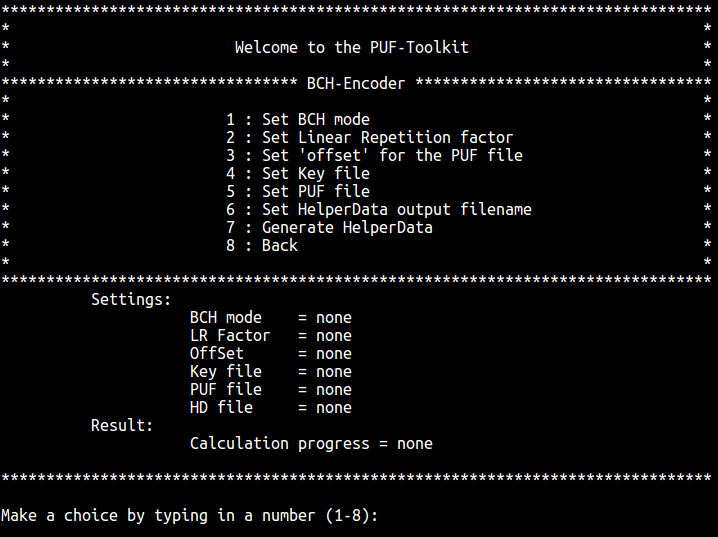
\includegraphics[width=0.9\textwidth]{images/bch_encoder_ui.png}}
\caption{Console user interface of the \emph{PUF BCH Encoder}.}
\label{img:4_BCH_ENC_menu}
\end{figure}
The User interface for the BCH Encoder sub menu is shown in Figure \ref{img:4_BCH_ENC_menu}. The first option is to set the BCH mode in which the user is required to input the codelength $n$ i.e. derived from $m$ such that $(2^{m-1} - 1) < length <= (2^m - 1)$, after that it is also mandatory to enter the desired correction capability $t$ of the BCH (n,k,d) code that in turn will determine the paramter $d$ of the code from the formula $t = \frac{d}{2} + 1$.
These values must be consistent with the equations \ref{4:BCH_len} and \ref{4:BCH_LR_len} or else the decoding of the secret key will not be successful. The second option chooses the LR factor as 7 or 15, the third is the familiar offsets selection for the PUF response that will also determine the actual length of the PUF response used to generate the helper data. After this the user must also input the key he/she wants to securely store and the name of the PUF
response file, finally the output filename for helperdata must be provided to be saved on permanent storage and to be used in the later reconstruction phase of the fuzzy extraction. These discussed inputs are all mandatory in the BCH menu and only then we can use option seven to process and generate the helper data or else the toolkit throws appropriate error messages to the user about missing parameters.\\

We show the functions of the BCH encoder arranged in modules that are related to each other via Figure \ref{img:bchenc_fns}

\begin{figure}
\centering
\fbox{ \includegraphics[width=0.9\textwidth]{images/bch_encoder_functions.pdf}}
\caption{Dependencies of the BCH Encoder Modules}
\label{img:bchenc_fns}
\end{figure}

The data structure \emph{Item} that was discussed in Hamming Distance contains relevant data members related to BCH encoder, which are summarized in the table \ref{tab:4_BCH_item_type_limits}

\begin{table}[!ht]
\begin{center}
\begin{tabular}{lll}
\toprule
\multicolumn{1}{l}{\textbf{Name}} & \multicolumn{1}{l}{\textbf{Type}} & \multicolumn{1}{c}{\textbf{Description}}\\
\midrule
\hline
\emph{offset\_begin} & long & \multicolumn{1}{l}{\begin{tabular}[l]{@{}l@{}}Defines the starting point in a binary file (bytes to skip from beginning) \end{tabular}}\\

\emph{offset\_end} & long & \multicolumn{1}{l}{\begin{tabular}[l]{@{}l@{}}Defines the ending point in a binary file (bytes to skip from end) \end{tabular}}\\

\emph{input\_Key\_length} & long & \multicolumn{1}{l}{\begin{tabular}[l]{@{}l@{}}Defines the length of the input key file\end{tabular}}\\

\emph{input\_Key\_name} & char [102] & \multicolumn{1}{l}{\begin{tabular}[l]{@{}l@{}}Char array for 102 symbols, to define the input key file \end{tabular}}\\

\emph{input\_PUF\_name} & char [102] & \multicolumn{1}{l}{\begin{tabular}[l]{@{}l@{}}Char array for 102 symbols, to define the input PUF file \end{tabular}}\\

\emph{output\_HD\_name} &  char [102] & \multicolumn{1}{l}{\begin{tabular}[l]{@{}l@{}}Char array for 102 symbols, to define the output helper data file \end{tabular}}\\

\emph{BCHmode} & char [25] & \multicolumn{1}{l}{\begin{tabular}[l]{@{}l@{}}Char array for 25 symbols, to define the BCH mode \end{tabular}}\\

\emph{LR} & int & \multicolumn{1}{l}{\begin{tabular}[l]{@{}l@{}}Definition of the utilized linear repetition factor \end{tabular}}\\

\emph{result} & char [52] & \multicolumn{1}{l}{\begin{tabular}[l]{@{}l@{}}Char array for 52 symbols, to provide feedback \end{tabular}}\\
\hline
\addlinespace
\bottomrule
\end{tabular}
\end{center}
\caption{Names and types of each element in the data structure \emph{Item} for the \emph{PUF BCH Encoder} and a description regarding their purpose.}
\label{tab:4_BCH_item_type_limits}
\end{table}

\subsubsection{Integration changes}
Initially the BCH Menu item was defined in the toolkit module to be called by the main menu, after that support for Offset from beginning and end, depicted in table \ref{tab:4_BCH_DEC_item_type_limits}, was made available similar to Hamming Distance menu. Since the ``Calculation module'' functions of the BCH encoder are all called internally without any dependence on the user, so they were unified with the original PUF Toolkit Calculation module without much hindrance.
The ``Settings module'' was merged to the toolkit with \emph{DefineFilename\_BCH} was renamed to avoid function name conflict with \emph{DefineFilename} of the toolkit, the former is dedicated to process the input PUF filename, output helperdata file and input secret key of the BCH encoder. The ``File and View modules'' were straightforward to unify with the toolkit, special care was taken to add the BCH global variables and global vectors to the toolkit. Changes in the ``View
module'' were dominated by the \emph{ErrorMessages} routine, which informs the user about the incorrect input and error states and the ways to recover from them. Major challenges faced during the integration were the same name functions as in the orignal toolkit that resulted in linking errors, they were resolved by renaming them appropriately for BCH encoder and all the declarations of the resulting functions were unified in the header files of the respective modules.\\

\subsubsection{Verification}
The correctness after merging the BCH encoder was authenticated via exhaustive run through all the test cases. In addition to that a final verification of the entire implementation was done. While doing the verification following main points were given priority:

\begin{itemize}
	\item Correctness of each module verified through utilization of test cases.
	\item All the possible menu options were checked and reviewed for their expected functionality
	\item Wrong inputs and incorrect state handling was also tested to make sure that the toolkit accepts only legitimate inputs and display appropriate error messages to rectify the error.
	\item Unusual workflows were inspected to assess their impact on Encoder functionality.
\end{itemize}

\subsection{PUF BCH Decoder}
We now go on to discuss the second phase of the fuzzy extractor i.e.``regeneration'' that uses PUF BCH Decoder as an essential element to recover the secret key that was encoded in the first phase with the help of the generated helper data and a PUF response from the same device as used in the enrollment phase. Again we do not indulge in the exact implementation details since they are presented with great detail in [Master seb thesis]. This section looks at the user interface of the BCH decoder where the possible inputs and their meaning is discussed, then a summary of the main modules involved in the BCH decoder
is presented with the help of an entity relation diagram. Similar to BCH encoder section we examine the changes required during merging with the toolkit in the subsection ``Integration Changes'' and finally talk about the verification steps taken to assert the correctness of the merged decoder functionality in the toolkit.\\

The decoder implementation is also the extension of the Morelos-Zaragozas [seb 43] but before applying the decoding functionality, the LR encoded helper data received from the first phase is processed in the majority vote module of the fuzzy extractor as shown in Figure \ref{img:4_MV_codewords}. This counteracts the linear repitition introduced in the LR coding module of the ``enrollment phase''. The fig. \ref{img:4_MV_codewords} shows this operation on the helper data received from fig. \ref{img:4_LR_HD}, notice that the PUF
response has some bits changed due to the various environmental factors (refer to section [2.1.4]) that introduce intra distance between the PUF reponses from the same device. After the Majority vote operation the BCH decoder recovers the configiration settings \emph{cfg} that are appended in the end of the helper data to satisfy correct boundary conditions as seen in the BCH encoding phase. Usually the BCH(n,k,d) can correct upto $t$ bit flip errors though along with Majority
Voting and BCH decoding the fuzzy extractor can restore the original input secret key.\\

The User interface is a simple GUI similar to the BCH encoder \ref{img:BCH_decoder_GUI}, but in this case the user need not enter the BCH mode details and offsets since they are predetermined in the encoding part and are saved as \emph{cfg} settings. We only need to give the helper data filename and the PUF response filename to decode and restore the input secret key. The output key filename is required to store the recovered input secret key and using option ``$5$'' the retrieved key can be viewed without
exiting the toolkit.\\

The five modules of the BCH decoder and their functions are depicted in the Figure \ref{img:bchdec_fns}.
\begin{figure}
\centering
\fbox{ \includegraphics[width=0.9\textwidth]{images/bch_decoder_functions.pdf}}
\caption{Dependencies of the BCH Encoder Modules}
\label{img:bchdec_fns}
\end{figure}

The members of the data structure \emph{Item} those are relevant to the BCH decoder are summarized in the table \ref{tab:4_BCH_DEC_item_type_limits}. The only difference with the encoder is that we need input helperdata filename instead of output helperdata filename and output key filename instead of the input key filename.

\begin{table}[!ht]
\begin{center}
\begin{tabular}{lll}
\toprule
\multicolumn{1}{l}{\textbf{Name}} & \multicolumn{1}{c}{\textbf{Type}} & \multicolumn{1}{c}{\textbf{Description}}\\
\midrule
\hline
\emph{offset\_begin} & long & \multicolumn{1}{l}{\begin{tabular}[l]{@{}l@{}}Defines the starting point in a binary file (bytes to skip from beginning) \end{tabular}}\\

\emph{offset\_end} & long & \multicolumn{1}{l}{\begin{tabular}[l]{@{}l@{}}Defines the ending point in a binary file (bytes to skip from end) \end{tabular}}\\

\emph{input\_HD\_name} &  char [102] & \multicolumn{1}{l}{\begin{tabular}[l]{@{}l@{}}Char array for 102 symbols, to define the input helper data file \end{tabular}}\\

\emph{input\_PUF\_name} & char [102] & \multicolumn{1}{l}{\begin{tabular}[l]{@{}l@{}}Char array for 102 symbols, to define the input PUF file \end{tabular}}\\

\emph{output\_Key\_name} & char [102] & \multicolumn{1}{l}{\begin{tabular}[l]{@{}l@{}}Char array for 102 symbols, to define the output key file \end{tabular}}\\

\emph{BCHmode} & char [25] & \multicolumn{1}{l}{\begin{tabular}[l]{@{}l@{}}Char array for 25 symbols, to define the BCH mode \end{tabular}}\\

\emph{LR} & int & \multicolumn{1}{l}{\begin{tabular}[l]{@{}l@{}}Definition of the utilized linear repetition factor \end{tabular}}\\

\emph{result} & char [52] & \multicolumn{1}{l}{\begin{tabular}[l]{@{}l@{}}Char array for 52 symbols, to provide feedback \end{tabular}}\\
\hline
\addlinespace
\bottomrule
\end{tabular}
\end{center}
\caption{Names and types of each element in the data structure \emph{Item} for the \emph{PUF BCH Decoder} and a description regarding their purpose.}
\label{tab:4_BCH_DEC_item_type_limits}
\end{table}

\subsubsection{Integration Changes}
To integrate the BCH decoder on top of already merged BCH encoder in the toolkit, required careful alterations to the code. The \emph{Main\_Menu} routine of the toolkit was modified to insert a BCH decoder menu that can be invoked by the user. The ``Calculation'' module functions were merged without much conflict with the existing functions, the function \emph{generate\_gf}, responsible for Galios Field computation was unchanged. The other two functions
\emph{read\_p\_decode and gen\_poly\_decode} that are used for polynomial generation were renamed because of the overlapping function names with the encoder. The error messages displaying routine of the ``View module'' was redeclared as  \emph{ErrorMessages\_decode} because the error states and the possible inputs for decoder are different from the BCH encoder. \emph{MajorityVoting} and \emph{ViewFile} were added to the family of BCH functions and correspondingly their declarations written in respective header files. The
routine \emph{DefineFilename\_BCH} was specifically modified to take two more arguments i.e. input helperdata filename and output recovered key name, since these two arguments were not implemented in the encoder. Accordingly the body of the same routine was changed to display appropriate messages for the input of helperdata and output key name that would be restored after decoding. The other challenge was to find and modify all the invoking points to the newly renamed functions, this was
resolved by careful code investigation and with the help of insight gained via compiler and linker errors.\\

\subsubsection{Verification}
For verifying the integrated BCH decoder a similar approach as BCH encoder was taken, the correctness was authenticated by running all the test cases that cover all the code flows including exceptions and error states. A final verification of the entire implementation was done by cross checking the recovered key with the original secret key.


\begin{itemize}
	\item Correctness of each module verified through utilization of test cases.
	\item All the possible menu options were checked and reviewed for their expected functionality
	\item Wrong inputs and incorrect state handling was also tested to make sure that the toolkit accepts only legitimate inputs and display appropriate error messages to rectify the error.
	\item Unusual workflows were inspected to assess their impact on Decoder functionality.
	\item The restored key was matched with the original secret key using the linux commandline utility ``diff''.
\end{itemize}

\subsection{Golay Encoder}
This section discusses the Golay Encoder that was integrated in the toolkit. We first discuss the user interface then look at the functions and modules of the Golay encoder followed by a basic description of the important routines in the code and then steps taken to verify the implementation.\\

\begin{figure}
\centering
\fbox{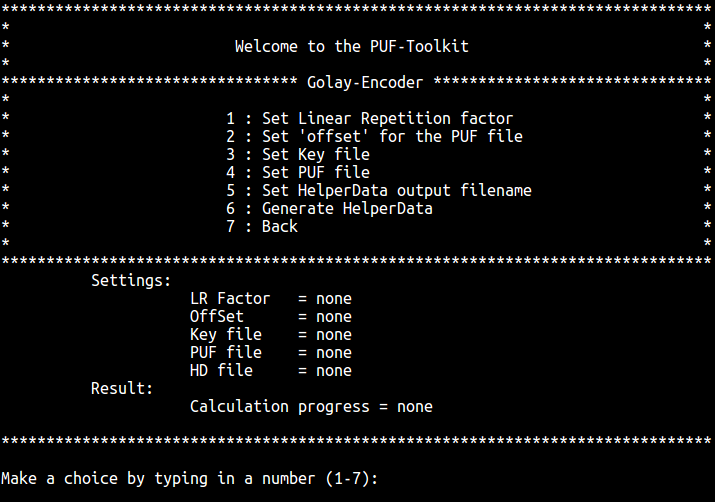
\includegraphics[width=0.9\textwidth]{images/golay_encoder_ui.png}}
\caption{Console user interface of the \emph{PUF Golay Encoder}.}
\label{img:golay_enc_ui}
\end{figure}
The UI is similar to BCH encoder but in this case we do not need to set the dimensions of the code ``n, k and d'' because Golay is a static code with the universal dimensions of (23, 12, 7) as seen in section \ref{golay_related}. The user interface is portrayed in Figure \ref{img:golay_enc_ui}, using the first option the user can set the Linear repetition factor as '7' or '15', the offsets of the PUF file can be adjusted using option two. After this it is mandatory to input the secret key filename, to be
stored securely, and input the PUF filename to generate the helperdata using fuzzy extractor algorithm, using option three and four respectively.The helperdata filename is provided by the user by selecting option five. If all the inputs are satisfied and conditions are met then the helperdata will be generated by choosing the last option six.\\


\begin{figure}
\centering
\fbox{ \includegraphics[width=0.9\textwidth]{images/golay_encoder_functions.pdf}}
\caption{Illustration of the Golay Encoder modules and their inter dependency.}
\label{img:golay_enc_funcs}
\end{figure}

The functions of the Golay Encoder are divided into four modules similar to the BCH encoder depicted in Figure \ref{img:golay_enc_funcs}. The \emph{Setting} module contains the familiar functions ``DefineFilename'' and ``DefineSettings'' alongwith ``DefineOffsetlength'' which sets the value of the offsets. The \emph{View} module contains the ``ErrorMessages'' routine which is implemented in the toolkit already to check for incorrect inputs by the user and other routines to check the progress status and
clear the screen. The \emph{Calculation} module forms the backbone of the golay encoder the details are listed below:

\begin{itemize}
	\item \emph{Golay\_encode} routine's main task is to read and allocate memory for the PUF and Key file using their filenames that are given by the user. This routines then makes a call to the ``generateHelperData'' function with the initialized data members of the Item structure and memory pointers to the read files.
	\item \emph{generateHelperData} generates the encoding table using another internal function \emph{get\_syndrome} (this table is analogous to the generator matrix discussed in section \ref{golay_related} of the Golay Code) , then the seret key is encoded using the Golay Coding technique. The generated Codewords are stored in an array that undergo the linear repetition process and finally the LR\_Encoded codewords are XORed with the PUF response to obatin the
		helperdata. The generatorHelperData stores the final output in the helperdata filename specified by the user alongwith the ``cfg'' settings i.e Offsets, LR factor and secret key filesize. This information will be read and used in the decoder module. Table \ref{tab:Golay_pattern} summarizes the data structure ``Pattern'' that constitute the cfg settings.

	\item \emph{get\_syndrome} function computes the generator polynomial for golay code corresponding to the (23, 12, 7) golay code. \end{itemize}

\begin{table}[!ht]
\begin{center}
\begin{tabular}{lll}
\toprule
\multicolumn{1}{l}{\textbf{Name}} & \multicolumn{1}{c}{\textbf{Type}} & \multicolumn{1}{c}{\textbf{Description}}\\
\midrule
\hline
\emph{errorCode} & int & \multicolumn{1}{l}{\begin{tabular}[l]{@{}l@{}}Defines the utilized error correction code (0 = Golay, 1 = BCH)\end{tabular}} \\

\emph{Golay\_BCH\_length} & int & \multicolumn{1}{l}{\begin{tabular}[l]{@{}l@{}}Defines the \emph{length} of one code word, for Golay and BCH \end{tabular}}\\

\emph{Goly\_d\_BCH\_t} & int & \multicolumn{1}{l}{\begin{tabular}[l]{@{}l@{}}Defines for Golay the distance \emph{d} and for BCH the correction capability '\emph{t}' \end{tabular}}\\

\emph{Golay\_k\_BCH\_m} &  int & \multicolumn{1}{l}{\begin{tabular}[l]{@{}l@{}}Defines the \emph{message length} for Golay and the parameter \emph{m} for BCH\end{tabular}}\\

\emph{linearRep} & int & \multicolumn{1}{l}{\begin{tabular}[l]{@{}l@{}}Defines the utilized linear repetition factor\end{tabular}} \\

\emph{puf\_offSet\_begin} & long & \multicolumn{1}{l}{\begin{tabular}[l]{@{}l@{}}Defines the starting point in a binary file (bytes to skip) from beginning \end{tabular}}\\

\emph{puf\_offSet\_end} & long & \multicolumn{1}{l}{\begin{tabular}[l]{@{}l@{}}Defines the ending point in a binary file (bytes to skip) from the end \end{tabular}}\\

\emph{original\_filesize} & long & \multicolumn{1}{l}{\begin{tabular}[l]{@{}l@{}}Defines the length of the original input key file \end{tabular}}\\
\hline
\addlinespace
\bottomrule
\end{tabular}
\end{center}
\caption{Names and types of each element in the data structure \emph{Pattern} for the \emph{PUF Golay Encoder} and a description regarding their purpose.}
\label{tab:Golay_pattern}
\end{table}

A helper function \emph{SetInputLen} was implemented to aid the encoder functions in calculating the length of the file based on the offsets. This function is called internally before reading and allocating the memory for key and PUF response. It takes two arguments, first the Item structure with intialized data members as filenames and a second integer argument that point to PUF response or secret key, based on these values it calculates the input length as $input\_length =
orignal\_filesize - (Offset\_end + Offset\_beginning)$. \\

\subsubsection{Verification}
The user interface was designed to follow the same pattern as BCH encoder to simplify the user experience. The ``Main'' module was modified to add one more menu item \emph{Golay\_Encoder\_Menu}. The merging and reuse of the existing functions was done with great care and detail to modularize the code that is suitable for further extension in the future. The verification of the consolidated code was done keeping in mind the the same steps as BCH encoder:
\begin{enumerate}
	\item Correctness of each module verified through utilization of test cases.
	\item All the possible menu options were checked and reviewed for their expected functionality
	\item Wrong inputs and incorrect state handling was also tested to make sure that the toolkit accepts only legitimate inputs and display appropriate error messages to rectify the error.
	\item Unusual workflows were inspected to assess their impact on Golay Encoder functionality.
\end{enumerate}

Due to the static nature of the Golay Code (23, 12, 7) it can only correct upto ``three errors'' per ``twelve bits'' of message. Consequently this code is not suitable for encoding and large secret files. Extensive testing showed that when the resultant helperdata is greater in size compared to the PUF response, the secret file is not recovered completely and via hit and trial the filesize for complete recovery of the secret key was approximated $2600$ bytes. So the recovery of ssh private keys which are
typically greater than 3000 bytes is not possible using Golay and the user must choose the BCH fuzzy extractor instead.

\subsection{Golay Decoder}
The next step after encoding the secret key and obtaining the helper data is to recover the key via golay decoding. The subtext presents the user interface and explains the procedure to restore the securely stored secret key, then the modules and functions of the decoder are illustrated. The discussion then follows the code improvement done to enhance the menu of the toolkit and finally verification strategy to check the integrated changes is shown.\\

The user interface \ref{img:golay_decoder_ui} has five main options where the user must input the helperdata that was generated in the enrollment phase using option one. The other two mandatory options are to set the PUF response filename that is generated from the same device as used in encoding phase and to specify the output key filename where the secret key will be restored. If all the inputs are correctly set then the ``regeneration'' can be performed via option four. The output and status is displayed
under the \emph{Result} section of the UI whereas \emph{Settings} subsection of the interface shows the filenames. If the input is incorrect or if the given filename is not present on the disk then a suitable error with details to recover from a faulty state is shown to the user.\\
\begin{figure}
\centering
\fbox{ 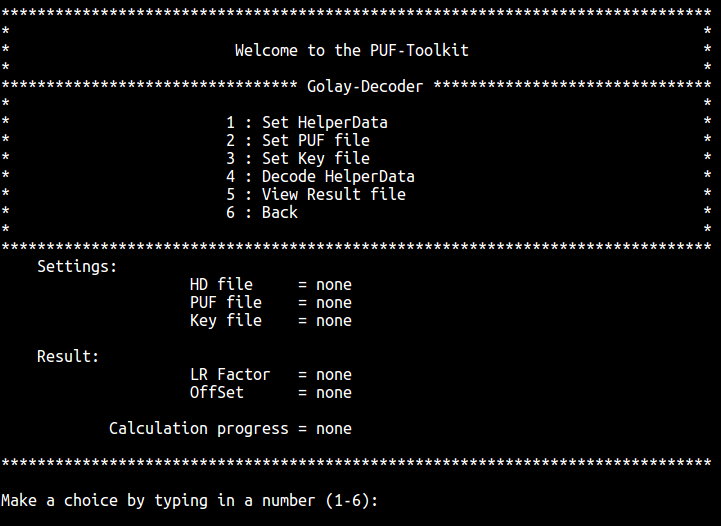
\includegraphics[width=0.9\textwidth]{images/golay_decoder_ui.png}}
\caption{Conceptual design of the Golay Deocder user interface.}
\label{img:golay_decoder_ui}
\end{figure}

\begin{figure}
\centering
\fbox{ \includegraphics[width=0.9\textwidth]{images/golay_decoder_functions.pdf}}
\caption{Illustration of the Golay Decoder modules and their inter dependency.}
\label{img:golay_decoder_ui}
\end{figure}

Golay decoder code is partitioned across five modules similar to the ones discussed in Golay encoder as illustrated in Figure \ref{}. The first module is the Main\_Menu function that calls the Golay decoder menu. This menu was implemented and added to the PUF toolkit which on selection points to the user interface with menu items of the decoder \ref{img:golay_decoder_ui}. The golay decoder user interface is implemented in the routine \emph{Golay\_Decoder\_Menu}, where the decode option is linked to the \emph{Golay\_decode}
function that performs the decoding of the helperdata. The usual routines in the ``View'' module are used to set the helperdata, PUF response and output recovered key filenames. There is no need to set the offsets and orignal key filesize in the decoder menu since during the ``enrollment'' phase these details are appended at the end of helperdata as part of the `cfg' settings. The ``Calculation'' module is crucial to the decoding operation and which follows the below mentioned
steps:
\begin{enumerate}
	\item The Golay decode function reads the `cfg' settings using a sub routine \emph{read\_infos} that reads the settings appended at the end of the helperdata and initializes the correspoding data members of the Item strucuture. The details of the data members used in golay decoding are listed in table \ref{tab:Golay_pattern}. Then based on the settings the input length of the PUF response is calculated as $input\_length = orignal\_filesize - (Offset\_end + Offset\_beginning)$. The files
		helperdata and PUF response are read and stored in the memory and the control is given to the \emph{recoverOriginalData}.
	\item The next function \emph{recoverOriginalData} performs the decoding of the helperdata. It first applies ``Majority Voting'' on the encoded helperdata to reverse the effects of the ``Linear Repetition'' done during enrollment phase. With the help of an api \emph{next\_comb} the decoding table for Golay code (23, 12, 7) is calculated that is used to recover the original key.
	\item After the restoration of the key is complete it is saved in the output key filename by calling a
		sub-routine \emph{SaveFile} that takes the recovered key (represented in code as a character array) and output filename as arguments and uses standard C file operations to write to the file.
\end{enumerate}

The \emph{ErrorMessages} function was used to detect incorrect input and display the errors to the user, since it is redundantly used in the other menu functionalities of the PUF toolkit like BCH encoder, we summarize the Error Codes in the table \ref{tab:Golay_dec_errors}

\begin{table}[!ht]
\begin{center}
\begin{tabular}{cp{13cm}}
\toprule
\multicolumn{1}{c}{\textbf{Error code}} & \multicolumn{1}{c}{\textbf{Error message}} \\
\midrule
\hline
1 & ERROR! Invalid input - Only digits are allowed! No digit at \emph{pos + 1}.\\

2 & ERROR! Invalid input - Input to long. \\

3 & ERROR! Invalid input - Try again...  \\

4 & ERROR! Opening output file. \\

5 & ERROR! Invalid input - 'Filename' too long. \\

6 & ERROR! Invalid input - No input. \\

7 & ERROR! Reading PUF file. \\

8 & ERROR! Opening PUF file. \\

9 & ERROR! Invalid input - PUF filename is not valid.\\

10 & ERROR! Invalid input - Key filename is not valid.\\

11 & ERROR! Opening HelperData file. \\

12 & ERROR! Reading HelperData file. \\

13 & ERROR! Selected an invalid choice. \\

14 & ERROR! HelperData: The recovered 'decoding information' is invalid! -> Parameter '\emph{m}' is out of range.\\

15 & ERROR! HelperData: The recovered 'decoding information' is invalid! -> Parameter '\emph{t}' is out of range.\\

16 & ERROR! HelperData: The recovered 'decoding information' is invalid! -> Parameter '\emph{length}' is out of range.\\

17 & ERROR! HelperData: The recovered 'decoding information' is invalid! -> Parameter '\emph{LR factor}' is not 7 or 15.\\

18 & ERROR! HelperData: The recovered 'decoding information' is invalid! -> Parameter '\emph{offSet}' is out of range.\\

19 & ERROR! HelperData: The recovered 'decoding information' is invalid! -> Parameter '\emph{filesize}' is out of range.\\

20 & ERROR! Opening file to view.\\

21 & WARNING! Looks like no decoding was performed.\\

22 & Looks like the calculation was not started.\\

23 & ERROR! Looks like the file was empty.\\

24 & ERROR! Looks like the file was not in the supported format.\\

25 & WARNING! Looks like the 'offset' is not set.\\

26 & ERROR! Looks like the 'Output file or Result' is not set/calculated.\\
\addlinespace
\bottomrule
\end{tabular}
\end{center}
\caption{Error codes and corresponding error messages for the \emph{PUF Golay Decoder}.}
\label{tab:Golay_dec_errors}
\end{table}

\subsubsection{Verification}
After the merging is complete and the Golay decoder menu is functional it was tested rigrously to make sure all the options work as expected. The same approach for verifiation was taken as mentioned in previous subsections and a final check was done to comapre the recovered key with the original secret to ensure the overall functionality of both the Golay encoder and decoder is correct.

\begin{itemize}
	\item Every menu item of the golay decoder was checked and review to make sure it behaves as expected.
	\item Incorrect inputs were inserted deliberiately to verify the ErrorMessages routine display corresponding error messages and ways to recover from the incorrect state of the toolkit.
	\item Unusual workflows were inspected to assess their impact on Encoder functionality.
	\item The recovered key was compared with the original secret key via the linux ``diff'' commandline utility and they were found to be identical.
\end{itemize}

\section{Jaccardi Index}
\label{jaccardi_index_section}
This section explains the Jaccardi Index implementation that was developed as a new feature for the toolkit. Then the two sub-menu options Intra Jaccardi and Inter Jaccardi Index are presented as subsections.
The modules and code structure was inspired from the Hamming Distance Menu since both of the metrics (Hamming Distance and Jaccardi Index) are closely related to each other and operate on either files or folders. We first discuss the definition of Jaccardi Index and its relation to the hamming weight. We then look at the user interface for the Jaccardi Index Menu which contains two more sub
menu options \emph{Inter} and \emph{Intra Jaccardi index} and then go on to explain the modules of the Jaccardi index. In the end the section presents the verification steps after the development of this new feature was complete.\\

\begin{itemize}
	\item \emph{Definition}: Jaccardi index between two bytes A and B is defined by the equation \ref{jaccard_eq}
	\begin{equation}
	J(A,B) = \frac {|A \cap B|} {|A\cup B|} = \frac{|A \cap B|} {|A| + |B| - |A \cap B|}
	\label{jaccard_eq}
	\end{equation}
	where |A| is the hamming weight of A, |B| is the hamming weight of B and $|A \cap B|$ is the number of times both A and B have one in the same bit position.
\end{itemize}

For eg. if we have two bytes A = 1100 1111 and B = 1111 0000 then |A| = 6, |B| = 4 and $|A \cap B|$ = 2 (since only first two common positions have ones in both the bytes). Substituting these values in the above equation we get $J(A,B) = (2) / ( 6 + 4 - 2) = 0.25$.\\

\begin{figure}
\centering
\fbox{ 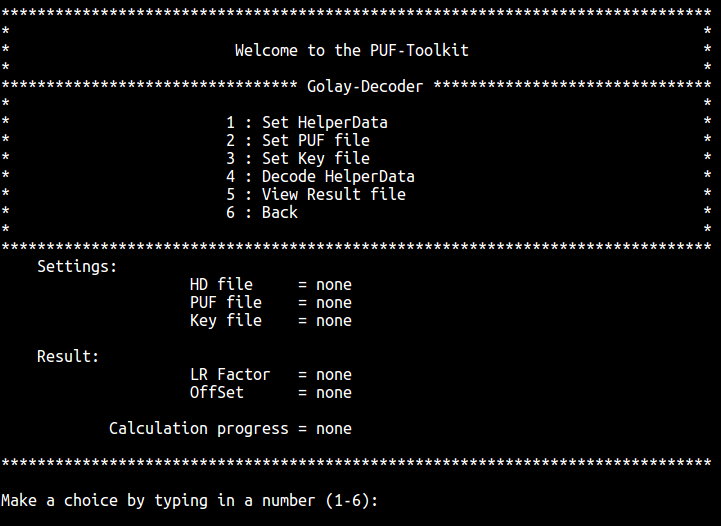
\includegraphics[width=0.9\textwidth]{images/golay_decoder_ui.png}}
\caption{Conceptual design of the Jaccardi Index user interface.}
\label{img:jaccard_ui}
\end{figure}
The user interface for the Jaccardi Index menu is similar to the Hamming Distance Menu as shown in Figure \ref{img:jaccard_ui}. Using the first option user can set the offsets from beginning and end of the file and as a result those bytes will be skipped during Jaccardi calculation. The second option lets the user set the output filename which is mandatory since the results will be stored in this file. The third option performs the computation of the Jaccard index between the two given
files. It first asks for the two filenames to be prompted by the user and then the result alongwith the \emph{Fractional Index} is stored in the output file. Option five and six calls the Intra and Inter Jaccardi Index routines respectively and are discussed in following subsections. The six and the last option can be used to view the output file without exiting the toolkit.\\

The modules of the Jaccardi's index are similar to those of the hamming Distance and therefore this section takes the liberty of not showing it here again.
Rather than looking at each and every module we look at the main routines and algorithm to calculate the Jaccardi Index.
\begin{itemize}
	\item The main Jaccardi index between two files is calculated by the \emph{Jaccard\_Index} that takes data structure Item pointer as an argument with initialized filenames. It first sets the input length of both the files based on the offsets from beginning and end by calling the \emph{SetInputLen} api which was designed specifically for this purpose.
	\item Then the files are read using the sub-routine \emph{readfile} that takes name of the file, offset from beginning and filesize as 		argument, based on that it reads and mallocs the file in memory and passes back the pointer to the allocated memory back to the caller function.
	\item To get the common number of ``1s'' at same bit positions in both the files, a bitwise AND operation is performed on the read files and the result is stored in a character array. The resultant character array contains the data with ``1s'' in the same bit position since bitwise AND operation only yeilds result ``one'' both the input bits are ``one''. This operation can be seen in the table \ref{bitwise_AND}.

\begin{table}[!ht]
\begin{center}
\begin{tabular}{lc}
\toprule
\multicolumn{2}{c}{\textbf{bitwise AND of two bytes A and B}}\\
\midrule
Byte A &   1100 0000 \\
Operation & \&\\
Byte B &   1111 0011 \\
Output C &   1100 0000 \\
\addlinespace
\bottomrule
\end{tabular}
\end{center}
\caption{bitwise ANDing the two bytes to get the common ones in the same bit position}
\label{bitwise_AND}
\end{table}

	\item Once the bitwise AND result is obtained then the calculation of Jaccardi Index is relatively simple. The number of ones in each input files and the bitwise ANDed output file are computed by calling the \emph{hamming\_wt} function explained in the section \ref{Hamming_Distance_menu} under listing \ref{lst:hammingwt} and then the values are substituted in the equation \ref{jaccard_eq}.
	\item An additional metric called Fractional Jaccardi's Index is also calculated using the definition $F(A, B) = J(A, B)/ size(A or B)$ and written to the result file alongwith the Jaccardi Index.
\end{itemize}

\subsection{Intra Jaccardi Index}
Instead of computing Jaccardi index between two files, the entire folder containing PUF responses from a single device can be evaluated by selecting the Intra Jaccardi Index sub-menu item. The filename where the results will be written is essential before processing the Intra Jaccardi Index. The menu item asks for an input directory with relative or absolute path on the machine and if the input path is correct and output file is set then the result is generated and stored in the
output file.\\

Contrary to the intra hamming distance the ``Switch output-style'' (refer section \ref{intra_hd_section}) option was not made available to the user to simplify the functionality. The default output-style was set as \emph{Compact} which is explained with detail in the Intra Hamming Distance section \ref{intra_hd_section} and illustrated in Figure \ref{img:4_intra_WP}. A sample result output file is presented in the Figure \ref{img:intra_jaccardi_compact} which shows the compact mode comparison between the files in the
directory where the Jaccardi Index in conjunction with fractional Jaccardi Index is written for each comparison.\\
\begin{figure}
\centering
\fbox{ 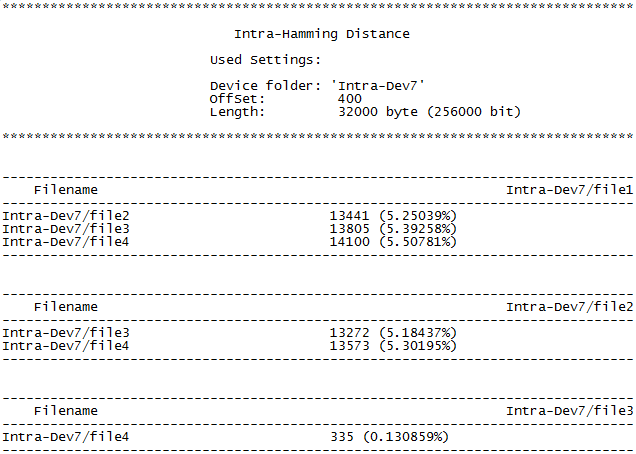
\includegraphics[width=0.9\textwidth]{images/4_intra_compact.png}}
\caption{A sample output result showing the \emph{compact} output style format for Intra Jaccardi Index }
\label{img:intra_jaccardi_compact}
\end{figure}

To realize the Intra Jaccardi Index the function \emph{Jaccard\_Intra} was implemented that takes the directory as input and first checks if the path is valid and there are more than one files present in the folder. Then all filenames with their absolute paths are stored in a standard C++ vector data structure. The \emph{Jaccard\_Intra} then iterates through this vector and computes the Jaccardi Index for each comparison by calling the \emph{Jaccard\_Index} procedure that was explained in the section
\ref{jaccardi_index_section}
above. Finally the result is written in each iteration of the loop and appended to the output file.\\

\subsection{Inter Jaccardi Index}
Unlike its Intra counterpart the Inter Jaccardi Index can be used to evaluate the PUF responses across different devices. It compares the PUF responses in a directory (analogous to a device since all PUF responses from a single device are stored in the same folder) to PUF responses in other directories. The comparison mode or the output-style by default is designed in the code to be ``compact'' since it simplifies the metric and also avoids any duplicate comparisons. The details of
the compact mode file comparison for Inter Jaccardi index are the same as for Inter Hamming Distance which are explained in detail in the section \ref{inter_hd_section} and the  compact comparison operation between three folders is shown in Figure \ref{img:inter_compact}.\\

The code implementation for Inter Jaccardi Index is achieved by the routine \emph{Jaccard\_Inter} which takes the data structure Item as an argument. The user needs to input the number of paths or folders he/she wants to evaluate, this number is bounded between \emph{two} and \emph{ninety-nine} i.e $2 <= n < 99$, then the folder names with their absolute or relative path are required by the toolkit. All these paths are verified by the code as valid and present in the memory, the
routine \emph{Jaccard\_Inter} verifies if each given folder has atleast one file. These folder names and paths are then stored in a standard C++ vector which is navigated in compact comparison fashion to compute the Jaccard Index. The nested for loop iterations are abstracted in this text to avoid complexity. In each iteration of the nested loop the comparison between PUF responses of different devices is achieved by redudant calls to the \emph{Jaccard\_Index} function explained in section
\ref{jaccardi_index_section} and result is written to the output file as specified by the user.\\

\subsection{Verification}
The merging of a new feature to the toolkit required careful testing to ensure correctness and exceptions to be handled gracefully. Some of the approaches were inspired from the fuzzy extractor testing and are summarized below:
\begin{itemize}
	\item All the menu item were checked and reviewed for their expected functionality.
	\item Testing was done for faulty and incorrect inputs to the Jaccardi Index menu options to ensure relevant error messages are displayed to the user. For eg. incorrect paths or filenames of the directories will be prompted to the user suggesting to enter the paths/filenames again.
	\item The Jaccardi output file was reviewed to check for proper header information and tables.
	\item For Intra and Inter Jaccardi index, mandatory option like setting of the offsets and the output file was checked before computing the index. Incase these settings are not configured then relevant error information was displayed to the user.
\end{itemize}

This marks the completion of the improvement and development phase of the toolkit. Next part of the report discusses the integration of the toolkit to the CogniCrypt opensource libarary by interfacing the C++ APIs to the Java runtime via Java Native Interface.

\section{CogniCrypt Integration}

To make the C++ source code functions available to the Java runtime they must be interfaced using the Java Native Interface Technology. This section looks at the details of the Java Native interface, most of which is inspired from [jni.pdf], then the code implementation for the JNI is explained. Next the wrapping procedure of the toolkit as a shared library and packaged as a Java Archive (JAR) to be externally linked by the Java source code is clarified. The next subsections describe the Congicrypt and its clafer model
alongwith the xsl coding techniques to generate the java biolerplate code to assists the java developers.

\subsection{Java Native Interface}
Java Native Interface standard and programming techniques are defined by Oracle\textsuperscript{TM} as a native programming interface which allows Java code that runs inside a Java Virtual Machine (VM) to interoperate with applications and libraries written in other programming languages, such as C, C++, and assembly [oracle docs]. The JNI does not impose any restriction on the implementation of the underlying Java Virtual Machine so the native code works irrespective of the Virtual machine.\\

To implement the JNI code a lot of help was taken from the tutorial [jni url], for each metric of the toolkit an api was desgined in accordance with the syntax of the JNI. The text explains the development process for a single metric Hamming Distance, these steps are applied to all the other metrics too. The toolkit.java source file was written containing the native interfaces to the functions in the PUF toolkit. For eg. Hamming weight functionality of the toolkit was available via a public \emph{native} java function \emph{hammingwt} that takes ``file/foldername'', ``output filename'' and ``mode''(file mode or folder mode) as arguments.  These native apis are the class member functions of the Java \emph{toolkit} class.\\

The compilation of the toolkit java source was performed resulting in the toolkit.class file. Next the header file to be included in the JNI C++ source code was generated using the ``javah'' utility. The resultant header file contains the syntatical prototypes of the C++ interface functions that must be implemented. Such a file with hamming distance metric is shown in listing \ref{lst:jni_header}.
\begin{lstlisting}[frame=single,language=C++,
commentstyle=\color{magenta},
backgroundcolor=\color{white},
keywordstyle=\color{blue},
stringstyle=\color{orange},
basicstyle = \ttfamily \color{black} \footnotesize,
caption={Auto generated header file showing the syntax for Java Native Interface function declarations} ,
label={lst:jni_header},
captionpos=b,
numbers=left]
/* DO NOT EDIT THIS FILE - it is machine generated */
#include <jni.h>
/* Header for class jni_toolkit */

#ifndef _Included_jni_toolkit
#define _Included_jni_toolkit
#ifdef __cplusplus
extern "C" {
#endif
/*
 * Class:     jni_toolkit
 * Method:    hammingwt
 * Signature: (Ljava/lang/String;Ljava/lang/String;Z)V
 */
JNIEXPORT void JNICALL Java_jni_toolkit_hammingwt
  (JNIEnv *, jclass, jstring, jstring, jboolean);
\end{lstlisting}

The \emph{Java\_jni\_toolkit\_hammingwt} interface first parses the arguments that it obtained from the java source code. It takes the jstring arguments file/foldername and output filename, and converts them into standard C character array using the standard JNI conversion function \emph{GetStringUTFChars}. The jboolean argument is implicitly an integer so it does not require any transformation. The code then initializes the ``Item'' data structure with these values and calls the \emph{HammingWeight(Item *, int )} function of the toolkit to compute the hamming distance of the file or the entire folder based on the value of $mode$.\\ 

The \emph{ErrorMessages} routine of the toolkit is used to inform the user about invalid inputs and faulty toolkit states. Since these inputs are passed from the java source as strings, the java developers can check at their end for the authenticity of the file/folder names and their path on the machine. Other metrics of the PUF toolkit like ``entropy'', ``median and average'' etc. are implemented similarly in the java source and C++ source code.\\

\subsubsection{Packaging in Java Archive}
The C++ JNI source code alongwith the entire PUF toolkit must be compiled and linked as a shared library since the Java source code calls the native functions from the shared library or shared object. Before packaging the shared library and other java related class files in a JAR file the toolkit must be compiled as a shared object file. This is achieved by compiling and linking the PUF toolkit with the
``-fPIC'' and ``-shared'' flag of the GNU g++ compiler. The resultant ``libtoolkit.so'' can then be packaged in a JAR file.\\

JNI standard provide the API \emph{System.loadLibrary} to load the shared objects or Dynamic-Link Libraries (dll) from the java source code, but the CogniCrypt project requires the shared libary and the java toolkit.class to be packaged in a JAR , so that they can be included in the project as an External Libarary. For this purpose, another class is needed that can extract the shared object from the JAR , load it using the standard JNI function and then delete before the Java runtime exits. Such
a wrapper class was already implemented by [Adam Heinrich] and after little changes it was tailored to meet the needs of this project. To know more details about the implementation of this java source please refer [NativeUtils.java].\\

Once the toolkit.class, NativeUtils.class and libtoolkit.so are compiled they are packaged as a JAR file which is exported in the CogniCrypt as an External Archive.

\subsection{CogniCrypt Clafer Model}
CogniCrypt was implemented as an Eclipse Plugin to support the Java developers to enable easier use of the Cryptographic APIs [cryp.pdf]. It helps the developers to:
\begin{itemize}
	\item Generate secure implementations for cryptograhic tasks like Data Encryption.
	\item Analyzes the Java code and alerts for insecurely used cryptographic APIs.
\end{itemize}

CogniCrypt supports various crypto tasks and for the PUF toolkit to be made available in the list, a new task ``Evaluation and Assessment of PUF responses'' was implemented. After selecting the task a few high level questions like if the developer want to evaluate PUF response from a single or multiple device as shown in Figure \ref{img:cogni_ques}, must be answered by the developers.\\

\begin{figure}
\centering
\fbox{ 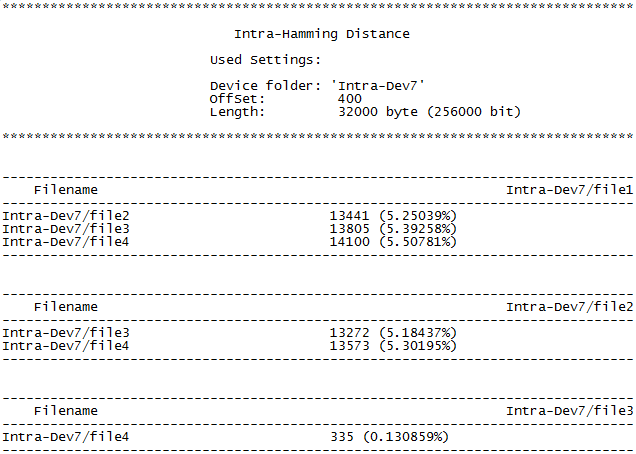
\includegraphics[width=0.9\textwidth]{images/4_intra_compact.png}}
\caption{An example of High level questions asked by the CogniCrypt for the Evaluating PUF responses}
\label{img:cogni_ques}
\end{figure}

Once all the questions are acknowledged, based on their answers the CogniCrypt presents a list of the algorithms that are eligible for selection for e.g if the developer answered evalution of PUF response from ``multiple devices'' then Inter Hamming Distance is only shown in the drop down since it is the only metric in the toolkit that takes more than one directory as input. In this case the CogniCrypt generates a java boilerplate code that shows the proper usage of the Inter Hamming Distance
function of the toolkit with directories (bounded between 2 and 99) as parameters to the API.\\

To achieve the above mentioned functionality the CogniCrypt employs a Clafer based model which is a lightweight modelling language that facilitates a mix of class and feautre modelling [clafer.org, cogni.pdf]. It supports constraint solvers that can generate instances of a model and satisfy its constraints [congi.pdf]. The answers to the high level questions determine the constraints on the model which is composed of different elements known as clafer. For the PUF toolkit each evaluation metric was
implemented as an clafer element and named as ``Metric'' in the model, one of the sample Metric is presented in listing \ref{lst:pufcfr}. \newpage

\begin{lstlisting}[frame=single,language=C++,
commentstyle=\color{magenta},
backgroundcolor=\color{white},
keywordstyle=\color{blue},
stringstyle=\color{orange},
basicstyle = \ttfamily \color{black} \footnotesize,
caption={Code snippet of a sample metric Hamming Distance in the PUF clafer model} ,
label={lst:pufcfr},
captionpos=b,
numbers=left]
abstract Metric
	description -> string
	fileMode -> FileMode
	devices -> Devices

Hamming_Distance : Metric
	[description = "hamming distance"]
	[fileMode = File || fileMode = Folder]
	[devices = Single]
\end{lstlisting}

The hamming distance extends the abstract Metric class that has two enums filemode and devices, and a string element as data members. These elements are initialized in the \emph{Hamming\_distance} class, lines 11-12 make ensures the hamming distance can only be evaluated for a file or an entire folder, such conditions are applied to other metrics too for eg. Inter Hamming distance must always evaluate for multiple devices.\\ 

After the clafer model is finalized and implemented, auto generation of the java code, that shows the developers the correct usage of the PUF toolkit functions, is achieved by the XSL stylesheet. For the PUF Toolkit the already implemented stylesheet in the CogniCrypt was enhanced to support the new functionality. Based on the answers by the developer to the high level questions the algorithm type or the metric is set in the clafer model which can be used in the <xsl if> statements
for matching and generating appropriate usage sample code. For eg. the listing \ref{ } shows the XSL stylesheet code to match the Hamming Distance metric and consequently produce java code that shows its proper usage.




\chapter{Evaluation}
\label{evaluation}
%The evaluation chapter covers the analysis of the integrated code and the improvements done to the toolkit and the evaluation of CogniCrypt interface to the toolkit. This analysis includes appraisal of the Design Guidelines and interpretation of the results of the metrics of the PUF toolkit for PUF response evaluation. The results of the measurements related to CPU usage and time requirements are presented as
histograms for better assessment of the number of CPU cycles used by the different metrics of the PUF toolkit. For fuzzy extractor techniques, the appraisal of the time requirement of the preprocessing  with respect to the parameter $m$ and a PUF response length analysis of the available BCH modes is given.\\

\section{Design Guidelines}
The user interface should be intuitive and easy-to-use which ensures user-satisfaction and effective use to the tool. While extending the toolkit and implementing new metrics, special consideration was given to the user interface design. The existing toolkit followed the standard guidelines as listed in \cite{67} and are summarized below:

\begin{itemize}
	\item \textbf{Simple and natural dialogue:} User must be provided with information related to the task such that the comprehension of the task is natural. The mapping of the user's mental model to the workflow of the toolkit has to be accurate. To satisfy this property the sub-menus are in a top-down structure i.e important options are always in the upper section of each menu. These options are also mandatory eg. the settings like offsets and file names must be set first before
		progressing to the calculation. The sub-menu items after calculation are optional, the toolkit menu follows a natural top-down workflow that is intuitive to the user and thus represents a simple and natural dialogue.
	\item \textbf{Speak the user's language:} The intended user group of the toolkit is assumed to be familiar with some technical vocabulary. Translating each and every instruction into layman's language distorts the meaning and is not always helpful. So all the dialogues are written as clear instructions with additional examples given to ensure a successful interaction between the user and the program.
	\item \textbf{Minimize the user's memory load:} To reduce retyping and user load, all the chosen settings are displayed in each menu. The long inputs like the paths to the different folders can be avoided via explained shortcuts. Common settings like offset needed to be set only once and are applied to all the sub-menus. Additionally, brief texts and guidelines to relax the short-term memory of the user are provided that promotes a clear design and visual clarity.
	\item \textbf{Be consistent:} The layout and positioning of the menu items, design concept is consistent throughout and wherever possible exact same words, menu entries, and settings options are used for the user to recognize a pattern and prediction of the actions. The control behavior is also consistent, meaning the upper area always shows the important options as mentioned in the text above.
	\item \textbf{Provide Feedback:} The information header in the toolkit informs the user where he/she is in the menu hierarchy. The Feedback and the input area provides with essential information about the result. Not only for errors, but feedback for each performed action and its status is displayed.
	\item \textbf{Provide clearly marked exits:} The ``exit'' or ``back'' is the lowest menu option in each sub-menu level. This facilitates user yo navigate through the hierarchical structure of the menu or to exit the toolkit.
	\item \textbf{Provide shortcuts:} The selection of each menu entry is implemented as shortcut represented by the corresponding number in front of the option. This helps is fast and spontaneous navigation through the menus.
	\item \textbf{Good error messages:} Whenever user input is incorrect or toolkit is in a faulty state, the reason for the error and information to recover from the erroneous state is given in the feedback area. The instructions are simplified and only relevant information to the error with as much detail as possible is presented thereby assisting user for a fast recovery.
	\item \textbf{Prevent errors:} The implementation has a two-level check for handling the user inputs to ensure that only legitimate inputs will be processed. Further information related to the input format and representative examples of such sample inputs with brief helper text is displayed to the user for him/her to avoid errors. Exhaustive error checking is performed before calculating the metric to assure that all relevant data and settings are set and valid, so as to prevent
		the program from running into undesired state and crashes.
\end{itemize}

\subsection{CogniCrypt User interface}
The CongniCrypt user interface consists of dialog boxes that ask simple questions to help the Java developers call the functions of the toolkit.
The above-mentioned design guidelines were considered for the development of the UI of CogniCrypt. They not only help to implement a secure Java code for the invocation of the toolkit functions but also assists the developers in getting familiar with the pattern of the toolkit and structure of the PUF responses. For eg. One major question asked by the CogniCrypt to the developer is if he/she wants to evaluate from a single PUF instance or multiple PUF instances (folders), for multiple
folders the CogniCrypts selects Inter-Hamming Distance. Such a question dialog box is represented in Figure \ref{img:cogni_ui} which shows the simple and intuitive design of the User Interface.\\

\begin{figure}
\centering
\fbox{ 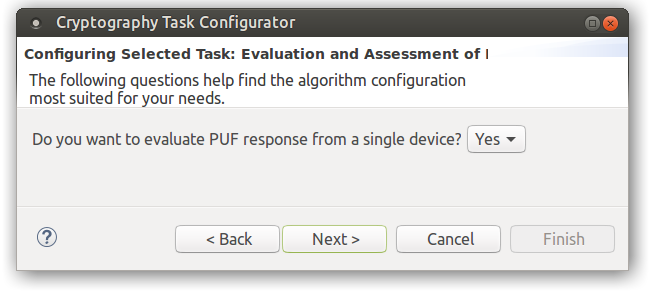
\includegraphics[width=0.97\textwidth]{images/Cogni.png}}
\caption{User interface of the CogniCrypt, represented as a dialog box that asks simple questions for the evaluation of the PUF metrics.}
\label{img:cogni_ui}
\end{figure}

During the testing of the CongiCrypt interface, a critical bug was discovered and resolved. If the absolute path of the file name exceeded a certain number of characters then the Toolkit crashed with a segmentation fault. The root cause was the generation of white space by calling the C++ API ``string'' that takes \emph{length} as one of the argument. But when the absolute path is very big the length becomes negative and Toolkit throws a runtime error.\\

To further enhance the developer experience and improve the UI a survey was taken and the suggestions of the Java developers were integrated into the CogniCrypt. For details of the survey please refer to the research paper \cite{crypto_icse}.

\begin{table}[!t]
\centering
\begin{tabular}{@{}lccccc@{}}
\toprule
\multicolumn{1}{l}{\textbf{Metric}}                                                                                             & \multicolumn{1}{c}{\textbf{Instance(s)}} & \multicolumn{1}{c}{\textbf{Challenge(s)}} & \multicolumn{1}{c}{\textbf{Ideal result}}                                         & \multicolumn{1}{c}{\textbf{Deviations}}                                            & \multicolumn{1}{c}{\textbf{Interpretation}}\\
\toprule
\midrule
\multicolumn{1}{l}{\begin{tabular}[c]{@{}l@{}}Hamming \\ weight\end{tabular}}                             & \multicolumn{1}{c}{-}                   & \multicolumn{1}{c}{-}                    & \multicolumn{1}{c}{\begin{tabular}[c]{@{}c@{}}(fractional) \\ 50\%\end{tabular}} & \multicolumn{1}{l}{\begin{tabular}[l]{@{}l@{}}minimal \\ acceptable\end{tabular}} & \multicolumn{1}{l}{\begin{tabular}[l]{@{}l@{}}PUF response \\unbiased\end{tabular}}      \\ \midrule
\multicolumn{1}{l}{\begin{tabular}[c]{@{}l@{}}(Shannon) \\ entropy\end{tabular}}                          & \multicolumn{1}{c}{-}                   & \multicolumn{1}{c}{-}                    & \multicolumn{1}{c}{1}                                                            & \multicolumn{1}{l}{\begin{tabular}[l]{@{}l@{}}minimal \\ acceptable\end{tabular}} & \multicolumn{1}{l}{\begin{tabular}[l]{@{}l@{}}Randomness of \\ PUF response\end{tabular}} \\ \midrule
\multicolumn{1}{l}{\multirow{2}{*}{\begin{tabular}[c]{@{}l@{}}Intra-\\ Hamming \\ distance\end{tabular}}} & \multicolumn{1}{c}{same}                & \multicolumn{1}{c}{same}                 & \multicolumn{1}{c}{\begin{tabular}[c]{@{}c@{}}(fractional) \\ 0\%\end{tabular}}  & \multicolumn{1}{l}{\begin{tabular}[l]{@{}l@{}}minimal \\ acceptable\end{tabular}} & \multicolumn{1}{l}{Reliability}                                                           \\ \cmidrule(l){2-6}
\multicolumn{1}{l}{}                                                                                      & \multicolumn{1}{c}{same}                & \multicolumn{1}{c}{different}            & \multicolumn{1}{c}{\begin{tabular}[c]{@{}c@{}}(fractional) \\ 50\%\end{tabular}} & \multicolumn{1}{l}{\begin{tabular}[l]{@{}l@{}}minimal \\ acceptable\end{tabular}} & \multicolumn{1}{l}{Uniqueness}                                                            \\ \midrule
\multicolumn{1}{l}{\begin{tabular}[c]{@{}l@{}}Inter-\\ Hamming\\ distance\end{tabular}}                   & \multicolumn{1}{c}{different}           & \multicolumn{1}{c}{same}                 & \multicolumn{1}{c}{\begin{tabular}[c]{@{}c@{}}(fractional)\\ 50\%\end{tabular}}  & \multicolumn{1}{l}{\begin{tabular}[l]{@{}l@{}}minimal\\ acceptable\end{tabular}}  & \multicolumn{1}{l}{Uniqueness}                                                            \\ \midrule
\multicolumn{1}{l}{\multirow{3}{*}{\begin{tabular}[c]{@{}l@{}}Min-\\ entropy\end{tabular}}}               & \multicolumn{1}{c}{same}                & \multicolumn{1}{c}{same}                 & \multicolumn{1}{c}{0}                                                            & \multicolumn{1}{l}{\begin{tabular}[l]{@{}l@{}}minimal \\ acceptable\end{tabular}} & \multicolumn{1}{l}{\begin{tabular}[l]{@{}l@{}}Robustness /\\Reliability\end{tabular}}    \\ \cmidrule(l){2-6}
\multicolumn{1}{l}{}                                                                                      & \multicolumn{1}{c}{different}           & \multicolumn{1}{c}{same}                 & \multicolumn{1}{c}{\begin{tabular}[c]{@{}c@{}}(fractional)\\ high\end{tabular}}  & \multicolumn{1}{l}{\begin{tabular}[l]{@{}l@{}}minimal\\ acceptable\end{tabular}}  & \multicolumn{1}{l}{Uniqueness}                                                            \\ \cmidrule(l){2-6}
\multicolumn{1}{l}{}                                                                                      & \multicolumn{1}{c}{same}                & \multicolumn{1}{c}{same}                 & \multicolumn{1}{c}{\begin{tabular}[c]{@{}c@{}}(fractional)\\ high\end{tabular}}  & \multicolumn{1}{l}{\begin{tabular}[l]{@{}l@{}}minimal\\ acceptable\end{tabular}}  & \multicolumn{1}{c}{\begin{tabular}[l]{@{}l@{}}Noise extraction\\ possible\end{tabular}}   \\
\midrule

\multicolumn{1}{l}{\begin{tabular}[c]{@{}l@{}}Jaccard \\ Index\end{tabular}}                             & \multicolumn{1}{c}{-}                   & \multicolumn{1}{c}{-}                    & \multicolumn{1}{c}{100\%} & \multicolumn{1}{l}{\begin{tabular}[l]{@{}l@{}}minimal \\ acceptable\end{tabular}} & \multicolumn{1}{l}{\begin{tabular}[l]{@{}l@{}}PUF response \\similarity\end{tabular}}      \\ \midrule
\multicolumn{1}{l}{\multirow{2}{*}{\begin{tabular}[c]{@{}l@{}}Intra-\\ Jaccard \\ Index\end{tabular}}} & \multicolumn{1}{c}{same}                & \multicolumn{1}{c}{same}                 & \multicolumn{1}{c}{\begin{tabular}[c]{@{}c@{}}(fractional) \\ 0\%\end{tabular}}  & \multicolumn{1}{l}{\begin{tabular}[l]{@{}l@{}}minimal \\ acceptable\end{tabular}} & \multicolumn{1}{l}{Reliability}                                                           \\ \cmidrule(l){2-6}
\multicolumn{1}{l}{}                                                                                      & \multicolumn{1}{c}{same}                & \multicolumn{1}{c}{different}            & \multicolumn{1}{c}{50\%} & \multicolumn{1}{l}{\begin{tabular}[l]{@{}l@{}}minimal \\ acceptable\end{tabular}} & \multicolumn{1}{l}{Uniqueness}                                                            \\ \midrule
\multicolumn{1}{l}{\begin{tabular}[c]{@{}l@{}}Inter-\\ Jaccard\\ Index\end{tabular}}                   & \multicolumn{1}{c}{different}           & \multicolumn{1}{c}{same}                 & \multicolumn{1}{c}{50\%}  & \multicolumn{1}{l}{\begin{tabular}[l]{@{}l@{}}minimal\\ acceptable\end{tabular}}  & \multicolumn{1}{l}{Uniqueness}                                                            \\ \midrule

\addlinespace
\bottomrule
\end{tabular}
\caption{Extended version of the table showing Interpretation of the results regarding the metrics in dependency to the utilized use case.}
\label{tab:metrics}
\end{table}

\section{Interpretation of the results for the extended metrics}
The interpretation for the core metrics that were implemented already in the toolkit is explained in detail in \cite{71}. This section presents the interpretation of the extended metrics and also touches upon the hamming weight interpretation since it is a base metric upon which other PUF evaluation metrics are built.
\begin{itemize}
	\item \textbf{Hamming Weight:} This metric was introduced in section \ref{Hamming_Distance_menu} and is used to ensure that a PUF response is not biased towards 0 or 1. For the result to be unbiased, the PUF response evaluation for the Fractional hamming weight metric between two files should be as close to 50\% as possible. Slight deviations are acceptable.
	\item \textbf{Jaccard Index:} This metric is also sometimes referred to as Jaccard similarity coefficient. As its alternate name suggests the Jaccard index measures similarity between two files so the Jaccard Index should be as close to $1$ or the $Jaccard Index * 100$ should be as close to 100\% as possible for two files to be similar.
	\item \textbf{Intra-Jaccard Index:} The general use case for evaluation of the Intra-Jaccard Index is when evaluating PUF responses from a single PUF instance with the same particular challenge. Ideally, the PUF responses from the same PUF instance and same challenge must be identical, but errors are introduced due to external factors like operating temperature change, voltage fluctuation etc. The PUF responses from the same PUF instance are stored in a particular directory and evaluation
		for intra-Jaccard Index is done for this entire folder. The result for each comparison should be close to $1$ which establishes similarity between files. The fractional Jaccard Index which is $Jaccard Index / filesize$ should be close to zero, considering the PUF response sizes are much greater than one byte. Note, slight deviations are tolerable. Another use case for this metric is to gain insight in the uniqueness of the PUF responses from a single PUF instance when
		it is stimulated with different PUF challenges. In such a case the resultant PUF responses should be different from each other depending on the PUF challenge. Note this evaluation only holds ground if the PUF instance offers a challenge space that is greater than one. In this case the Jaccard Similarity Index should be around $0.5$ (or 50\%) which establishes exclusiveness amongst PUF responses.
	\item \textbf{Inter-Jaccard Index:} Contrary to the Intra-Jaccard Index where evaluation of the PUF responses from a single device is done, Inter-Jaccard Index evaluates PUF responses from multiple devices. As stated above each PUF instance stores the responses in a specific directory, so multiple directories represent multiple PUF instances containing PUF responses which ideally must be similar within the same directory but must be unique and exclusive amongst other directories.
		Therefore the inter Jaccard Index for the same PUF challenge to different PUF responses from
		separate PUF instances should be as close to $0.5$ (or 50\%) as possible to ascertain
		uniqueness. Slight deviations from this ideal number are always acceptable.
\end{itemize}

For completeness table \ref{tab:metrics} summarizes the result interpretation of the metrics with respect to the utilized use case. The table also contains metrics from the original toolkit and are not explained in detail to avoid redundancy. To know more about the metrics in the previous version of the toolkit refer to \cite{71}.\\

\textbf{Time requirements:} To test the new metrics of the toolkit an analysis of the time taken by the calculation APIs for the PUF response evaluation of multiple instances was performed. The time taken by the user to input the settings was skipped, the measurement of the time was done using the standard ``clock()'' API of the GNU C library which is used to determine the process time. For testing, the SRAM PUF responses from Texas Instrument (TI) Stellaris LM4F120XL LaunchPad Evaluation Kits with a
size of 32 Kilobytes and an offset of 400 bytes from the beginning was used. The analysis was performed on an Intel i3 quad core CPU with 2.00 GHz and 3 GB RAM. The results of the time requirements for Intra Jaccard Index and Inter Jaccard Index are visualized in Figures \ref{img:time_intra} and \ref{img:time_inter} respectively. Figures \ref{img:cpu_intra} and \ref{img:cpu_inter} show the average percentage of CPU usage for Intra and Inter-Jaccard Index with the same parameters. The time taken analysis for the Jaccard Index is not represented since it is constant around $0.7$ milliseconds.
\vspace*{1.5\baselineskip}

\begin{figure}[h]
\centering
\fbox{ \includegraphics[width=0.875\textwidth,keepaspectratio]{images/intra_time.pdf}}
\caption{Time requirement measurements of the \emph{Intra-Jaccard Index} with PUF response of 32 kilobytes.}
\label{img:time_intra}
\end{figure}


\begin{figure}[t!]
\centering
\fbox{ \includegraphics[width=0.875\textwidth,keepaspectratio]{images/inter_time.pdf}}
\caption{Time requirement measurements of the \emph{Inter-Jaccard Index} with PUF response of size 32 kilobytes.}
\label{img:time_inter}
\end{figure}

\begin{figure}[h!]
\centering
\fbox{ \includegraphics[width=0.875\textwidth,keepaspectratio]{images/intra_cpu.pdf}}
\caption{Visualization of CPU usage by the \emph{Intra-Jaccard Index} for folders containing multiple PUF response of size 32 kilobytes.}
\label{img:cpu_intra}
\end{figure}

\newpage
\clearpage

\begin{figure}[t!]
\centering
\fbox{ \includegraphics[width=0.875\textwidth,keepaspectratio]{images/inter_cpu.pdf}}
\caption{Visualization of the CPU usage by the \emph{Inter-Jaccard Index} between mutiple folders containing multiple PUF response of size 32 kilobytes.}
\label{img:cpu_inter}
\end{figure}

\subsection{Evaluation of the Fuzzy extractor}

To evaluate the fuzzy extractor we compare both the coding techniques, Golay Code and BCH code used in the fuzzy implementation. Both of which are assisted with linear repetition algorithm and majority voting procedure. The error correction capability $t$ of Golay code is limited to a maximum of three-bit errors for a message length of \emph{12 bits}. Both the codes are linear codes so they take the same parameters (n, k, d), where $n$ is the length (in bits) of the encoded codeword, $k$ is the
length (message length) of the input secret/message that is fed to the encoder and $d$ is the minimal hamming distance from which the error correcting capability is derived using the formula $t = \lfloor(d-1)/2\rfloor$. The Golay code uses a lookup table to encode the \emph{12 bits} of message to \emph{23 bits} of codeword, in case there are more than three bits of errors introduced while processing PUF instance for response (due to external noise and environmental factors) then the decoding lookup
table for Golay code is not capable to correct errors which leads to an undesired state. To avoid this behavior, the user is presented with an error message that it is out of Golay code's scope to correct so many errors and to use BCH coding instead.

The BCH coding implementation, on the contrary, corrects as many bit errors as possible in each codeword. If errors exceed the correction capability $t$ of the BCH code then only $t$ errors are corrected and remaining errors are ignored. This avoids the undesired behavior unlike the Golay code and the information about the detected but not corrected errors is displayed to the user which enhances the robustness of the fuzzy extractor. In addition, the parameters of the BCH code are
highly configurable and can be adjusted to the noise level that introduces the errors. The pre-evaluation of the PUF responses from the PUF instances can be utilized to predict the error correction capability and the parameters of the BCH code can be adjusted accordingly to ensure a reliable working procedure. Table \ref{tab:BCHmodes} list the possible parameters that are valid for the BCH(n, k, d) code.\\

\begin{table}[!ht]
\small
\begin{center}
\begin{tabular}{rrrr|rrrr|rrrr|rrrr}
\toprule
\multicolumn{16}{c}{\textbf{Common BCH codes of order less than $2^{10}$}}\\
\midrule
\hline
n & k & d & t & n & k & d & t & n & k & d & t & n & k & d & t \\
\hline
7&4&3&1&127&8&63&31&511&484&7&3&511&166&95&47\\
15&11&3&1&255&247&3&1&&475&9&4&&157&103&51\\
&7&5&2&&239&5&2&&466&11&5&&148&107&53\\
&5&7&3&&231&7&3&&457&13&6&&139&109&54\\
31&26&3&1&&223&9&4&&448&15&7&&130&111&55\\
&21&5&2&&215&11&5&&439&17&8&&121&117&58\\
&16&7&3&&207&13&6&&430&19&9&&112&119&59\\
&11&11&5&&199&15&7&&421&21&10&&103&123&61\\
&6&15&7&&191&17&8&&412&23&11&&94&125&62\\
63&57&3&1&&187&19&9&&403&25&12&&85&127&63\\
&51&5&2&&179&21&10&&394&27&13&&76&171&85\\
&45&7&3&&171&23&11&&385&29&14&&67&175&87\\
&39&9&4&&163&25&12&&376&31&15&&58&183&91\\
&36&11&5&&155&27&13&&367&33&16&&49&187&93\\
&30&13&6&&147&29&14&&358&37&18&&40&191&95\\
&24&15&7&&139&31&15&&349&39&19&&31&219&109\\
&18&21&10&&131&37&18&&340&41&20&&28&223&111\\
&16&23&11&&123&39&19&&331&43&21&&19&239&119\\
&10&27&13&&115&43&21&&322&45&22&&10&255&127\\
&7&31&15&&107&45&22&&313&47&23&1023&1013&3&1\\
127&120&3&1&&99&47&23&&304&51&25&&1003&5&2\\
&113&5&2&&91&51&25&&295&53&26&&993&7&3\\
&106&7&3&&87&53&26&&286&55&27&&983&9&4\\
&99&9&4&&79&55&27&&277&57&28&&973&11&5\\
&92&11&5&&71&59&29&&268&59&29&&963&13&6\\
&85&13&6&&63&61&30&&259&61&30&&953&15&7\\
&78&15&7&&55&63&31&&250&63&31&&943&17&8\\
&71&19&9&&47&85&42&&241&73&36&&933&19&9\\
&64&21&10&&45&87&43&&238&75&37&&923&21&10\\
&57&23&11&&37&91&45&&229&77&38&&913&23&11\\
&50&27&13&&29&95&47&&220&79&39&&903&25&12\\
&43&29&14&&21&111&55&&211&83&41&&893&27&13\\
&36&31&15&&13&119&59&&202&85&42&&883&29&14\\
&29&43&21&&9&127&63&&193&87&43&&873&31&15\\
&22&47&23&511&502&3&1&&184&91&45&&863&33&16\\
&15&55&27&&493&5&2&&175&93&46&&858&35&17\\
\hline
\addlinespace
\bottomrule
\end{tabular}
\end{center}
\caption{BCH codes generated by primitive elements of order less than $2^{10}$ and the corresponding parameters \emph{n}, \emph{k} \emph{d} and \emph{t}.}
\label{tab:BCHmodes}
\end{table}

\subsection{Pre-evaluation Relevance}
\emph{\textbf{PUF response length analysis:}} To select the optimal BCH mode parameters it is important to ascertain the length of the PUF response which also forms a part of the pre-evaluation phase. The PUF response length is based on the size of the input secret and parameters $k$ and $d$ of the BCH code along with the Linear repetition factor selected for encoding. The PUF response length that satisfies the BCH code selection parameters can be verified using Equation
		\ref{PUF_length}.
\begin{itemize}
	\item The size of the input secret is $N$ bits, the BCH parameters corresponds to the chosen BCH(n, k, d) mode and the linear repetition factor is denoted with LR (7 or 15). The required length of the PUF response is represented with the symbol \emph{RequiredPUFLength}\cite{71}.\\
		\begin{equation}
			RequiredPUFLength \geq \Bigg\lceil\Bigg(\dfrac{\Bigg(\Bigg\lceil\dfrac{N}{k}\Bigg\rceil
		* n\Bigg)}{8}\Bigg)\Bigg\rceil * LR
		\label{PUF_length}
		\end{equation}
\end{itemize}

The pre-evaluation is inevitable for an effective and efficient development of PUF-based security approaches and it should be included in the development cycle of the PUF-based security algorithms. The pre-evaluation of the TI Stellaris LM4F120XL Launchpad Kit showed that the complete SRAM from this hardware cannot be considered as a PUF, because of the boot process which affects the randomness of the first  $400$ bytes and renders these bytes not to be considered a part of the PUF response.
Without pre-evaluation such exceptional behavior might not be discovered which can result in an insecure implementation of the PUF-based security approaches. For determining the required error correction capability of the BCH code, the pre-evaluation of the PUF instance is critical for the selection of the optimal parameters. These two scenarios illustrate that the pre-evaluation must be considered as a decisive factor in the development of the PUF-based security approaches.


\section{Time requirement analysis}

The BCH code is highly configurable that means the parameters m, n, t can be constructed in various possible ways. For time requirement analysis the preprocessing time for the generation of a BCH mode was taken into account. Depending on the selected parameters, specifically $m$, the preprocessing can create some timing overhead. Since this process is inevitable for both encoder and decoder, the timing overhead is considered with respect to the selection of the parameters, especially since
the adaptation of the fuzzy extractor is intended for hardware machine with limited resources. For testing, all possible m (in the range [4,14]), the corresponding maximum n ( $2^{n-1} - 1 < n <= 2^{n} - 1$) and the highest possible error correction capability t were chosen. The time requirement analysis was performed on an Intel i3 quad core CPU with 2.0 GHz and 3 GB RAM. The results of the time measurements for the BCH mode pre-processing are visualized in Figure \ref{img:bch_time}.
\begin{figure}[h]
\centering
\fbox{ \includegraphics[width=0.97\textwidth]{images/bch_preprocess.pdf}}
\caption{Time requirement measurements for the BCH mode pre-processing in relation to parameter m.}
\label{img:bch_time}
\end{figure}

\begin{figure}[h]
\centering
\fbox{ \includegraphics[width=0.97\textwidth]{images/golay.pdf}}
\caption{Time requirement measurements for the Golay encoding and decoding for varying filesizes}
\label{img:golay_time}
\end{figure}
The Golay code is a static (23, 12, 7) code where the user is not required to input any parameters. The pre-processing time of the Golay code remains constant and is not a timing overhead, so it can be ignored. The time required for encoding and decoding steps depends on the size of the file that is to be encoded/decoded. For the analysis, we used a PUF response from (TI) Stellaris LM4F120XL LaunchPad Evaluation Kits and the size was varied with the help of offsets, the original size of
the PUF response was 32 Kilobytes. Figure \ref{img:golay_time} illustrates the encoding and decoding analysis of Golay code with different file sizes as a bar graph.\\


\chapter{Conclusion}
\label{conclusion}
%\section{PUF Toolkit}
In this work, an already developed software-based toolkit named \emph{PUF Toolkit} was improved upon and extended. The implementation boosts the easy-to-use console user interface and provides the implementation of new common and proven metrics for the evaluation of the PUF responses. (To be specific the following metrics were added to the toolkit: \emph{Jaccard Index (Intra-Jaccard Index, Inter-Jaccard Index)} and \emph{Hamming Distance}. The implementation of the metrics favored an
	object-oriented approach and hence the toolkit was designed in C++ and to ensure an effective and intuitive working with the toolkit the user interface was derived from the nine main design guidelines by Nielsen and Molich\cite{67}. To support the designers and researchers in the evaluation of the PUF responses, the visualization of the metrics results was optimized with respect to PUF responses. The toolkit's functionality was enhanced to also skip bytes from the end of the PUF response
	(using an offset) and menu items were rearranged for better navigation. Apart from
these optimizations, the visual layout of the result file was improved to contain new parameters like offset from the end of the file, fractional Jaccard Index and Fractional Hamming Distance. A consistent development cycle and verification phase was performed for each metric implementation. The evaluation explained the interpretation of the results for the extended metrics and summarized already implemented metrics in a table. The user interface design guidelines were outlined
and a resource-friendly working of the toolkit was presented and finally the testing of the toolkit was done with a large set of samples and the data was recorded and visualized as bar graphs.\\

\section{Extension and Integration of Fuzzy Extractor}
The already implemented BCH code-based fuzzy extractor was added and integrated to the PUF Toolkit. The implementation of the fuzzy extractor was realized in C++ and it achieves a PUF-based secure key storage on hardware devices with limited resources. The integration part covered the combining of the data structures of the already implemented BCH code (based on Morelos-Zaragoza Encoder/Decoder for binary BCH codes in C \cite{69}) to the structure of the PUF Toolkit. Intensive code review was
done to correct some errors in the original Morelos-Zaragoza's implementation to ensure that the encoder and decoder functionalities work even with large values of parameter $m$. The erroneous state recovery, error correction capability and other functionalities of the PUF Toolkit were merged to the fuzzy extractor. The PUF BCH Encoder represents the enrollment phase of the fuzzy extractor for the realization of PUF-based secure storage. The BCH code is highly configurable and the code
parameters (n, k, d) along with error correcting capability $t$ and parameter $m$ can be adjusted according to user needs and PUF properties of the desired PUF instance. The BCH codes create code words which are processed by a linear repetition code before the result is ``one time encrypted'' with an XOR operation with the PUF response. The Encoder menu adheres to the above-mentioned design guidelines and provides an easy-to-use and well-structured user interface. The PUF BCH decoder
implementation is the counterpart of the PUF BCH Encoder and represents the second (reconstruction) phase of the fuzzy extractor. The reconstruction phase of the fuzzy extractor combines XOR operation with the PUF response and subsequently executes Majority Voting algorithm followed by the BCH decoder functionality to retrieve the original secret data. The integration procedure of the BCH decoder to the toolkit was similar to the integration procedure of the BCH encoder to the toolkit. The sub-menu of the
decoder is intuitive and a well-structured user interface that is inspired by the BCH encoder menu. The factors of the linear repetition code and the majority vote can take the value 7 or 15. For evaluation, the BCH fuzzy extractor was tested with different code parameters and the time requirements for the pre-processing step that creates a timing overhead were recorded and visualized as a time chart. The recovered file was cross-checked with the original secret making sure they were
identical.\\

The toolkit was extended with the Golay-based Fuzzy extractor. The original implementation of the Golay code was in a very basic format which hardcoded the input file, PUF response and other data structures, and had a very restrained functionality with no support for offsets, error recovery and user files input. All these functionalities were first added to the base version and then both the encoder and decoder parts of the Golay-based Fuzzy extractor were integrated to the PUF Toolkit. The
Golay encoder forms the generation phase of the fuzzy extractor. Similar to BCH encoder, it performs an XOR operation of the secret key with the PUF response and then applies linear repetition algorithm followed by Golay encoding to generate the helper data that is used in the decoding phase to recover the encoded secret key. But unlike BCH code, the parameters of the Golay code are fixed to (23, 12, 7); due to this limitation the recovery of large files that resulted in a helper data bigger than
the PUF response is not possible and the user is suggested to use BCH-based fuzzy extractor instead. The encoder also appends the configuration settings like offsets, input filesize and linear repetition factor to the helper data. The Golay decoder constitutes the reconstruction phase of the fuzzy extractor. It reads the saved configuration settings from the end of the helper file and then proceeds to an XOR operation of the helper data with the PUF response followed by the Majority Voting procedure with the same factor as the one used in by the linear repetition algorithm in the encoder part. Lastly based on the settings and code parameters (n, k, d) the decoder creates a decoding table and restores the original secret from the helper data, thus completing the PUF-based secure storage recovery. The menus for both encoder and decoder are derived from the BCH-based fuzzy extractor and
adhere to the same design guidelines as the PUF Toolkit, thereby making its user interface easy-to-understand and well-structured. The evaluation of the Golay code was done by testing the encoder and decoder for their time requirements and CPU usage with different PUF response sizes by adjusting the offsets and represented as a bar graph for analysis. A final check was performed using the ``diff'' utility to ensure that the recovered file does match the original input secret key.

\section{Integration to the CogniCrypt}
The metrics of the toolkit were made available to the Java developers for evaluation of PUF responses via the opensource library CogniCrypt. Using this library the developers with no prior knowledge about the PUF Toolkit can develop programs in Java by calling the functions of the toolkit. This was made possible by developing a separate module to interface the C++ code with the Java runtime via the Oracle Standard technology Java Native Interface. JNI is a programming
framework that enables the Java virtual machine to call the functions of the native applications and libraries written in other languages like C, C++, and assembly. The JNI enabled toolkit is compiled as a shared library and packaged as a JAR (Java Archive) to be included in the Java project as an external library for development. The CogniCrypt is an opensource library \cite{cogni} based on the Clafer lightweight modeling language \cite{clafer} and was developed to assist Java developers for secure and correct usage of the cryptographic APIs. It asks
simple questions from the developers to select the appropriate algorithm based on the answers and generate a boilerplate code that shows the sample usage of the cryptographic API. For this thesis the specific metrics of the PUF Toolkit namely: \emph{Hamming Weight, Intra-Hamming Distance, Inter-Hamming Distance, (Shannon) Entropy, min-Entropy} and \emph{median and average} were implemented as clafer algorithms and added to the CogniCrypt model. The graphical user interface of the
CogniCrypt is based on the advice taken from a survey, done with Java developers as the audience, on how to improve the usability of cryptographical APIs. Thus making it simple, intuitive and easy to use.\\

The extended and improved \emph{PUF Toolkit} integrated with the \emph{Fuzzy Extractor} functionality and interfaced to the \emph{CogniCrypt} opensource library, contributes to and accelerates the development of new security approaches. On one hand, it is helpful in the evaluation of PUFs in the context of security applications and on the other hand, it provides its functionalities to be used in a Java project and can be further used to realize new or enhanced security techniques that
are based on PUFs. Although there might be additional aspects that could be optimized in the future to further increase the PUF Toolkit application area, this thesis enhances the scope of the initial \emph{PUF Toolkit} to assist the researchers and developers in the evaluation of PUF instances.




\nocite{*}
bibliographystyle{ieeetr}
\bibliography{bibliography}
\end{document}
